\documentclass[11pt,a4paper]{article}

\usepackage[T1]{fontenc}
\usepackage[utf8]{inputenc}
\usepackage[french]{babel}
\usepackage{lmodern}
\usepackage[margin=2.4cm]{geometry}
\usepackage{microtype}
\DisableLigatures[-]{encoding=T1, family=tt*}
\usepackage{amsmath}
\usepackage{booktabs}
\usepackage{tabularx}
\usepackage{array}
\usepackage{xcolor}
\usepackage{graphicx}
\graphicspath{{../../bases/fpga/figures/}}
\usepackage{listings}
\usepackage{tikz}
\usetikzlibrary{positioning,arrows.meta,fit,babel}
\usepackage{csquotes}
\usepackage[round,authoryear]{natbib}
\usepackage[hidelinks]{hyperref}

\newcommand{\cmd}[1]{\texttt{#1}}
\definecolor{glcolor}{RGB}{0,95,115}
\newcommand{\gl}[2]{\hyperlink{gl:#1}{\textcolor{glcolor}{#2}}}
\newcommand{\nr}{\gl{nr}{\texttt{n/r}}}
\newcolumntype{L}{>{\raggedright\arraybackslash}X}

\definecolor{codebg}{gray}{0.96}
\lstset{
  basicstyle=\ttfamily\scriptsize,
  backgroundcolor=\color{codebg},
  frame=single, rulecolor=\color{gray!40},
  columns=fullflexible, keepspaces=true,
  breaklines=true, breakatwhitespace=false,
  postbreak=\mbox{\textcolor{gray}{$\hookrightarrow$}\space},
  showstringspaces=false,
  literate={é}{{\'e}}1 {è}{{\`e}}1 {à}{{\`a}}1 {É}{{\'E}}1
           {«}{{\guillemotleft}}1 {»}{{\guillemotright}}1 {…}{{\ldots}}1
}

\title{\textbf{PaperDatabase} : une base de connaissance textuelle et vérifiable\\
  pour la lecture assistée d'articles scientifiques}
\author{Léonard Rivals \and Maksym Lytvynenko}
\date{3 octobre 2026}

\begin{document}
\maketitle

\begin{abstract}
Préparer une thèse suppose de lire, comparer et citer des dizaines d'articles. Un grand
modèle de langage (\gl{LLM}{LLM}) peut aider, mais il travaille mal sur des \gl{PDF}{PDF} bruts : il en relit le
texte intégral à chaque question, ne sait pas où chercher un chiffre et mélange ce que dit un
article avec ce qu'il en déduit. PaperDatabase convertit chaque PDF en fichiers texte
structurés (métadonnées, sections paginées, références, \gl{fiche}{fiche} de lecture, tableau de
benchmarks) qu'un \gl{agent}{agent} LLM, ici Claude Code, parcourt du résumé vers le détail. Une couche
de recherche de \gl{passage}{passages}, de type \gl{RAG}{RAG}, s'y ajoute : \gl{index}{index lexical} \gl{BM25}{BM25} et index dense
(bge-small-en-v1.5) fusionnés par Reciprocal Rank Fusion, avec \gl{reranking}{reranking} optionnel. Cette
couche ne génère rien. Elle renvoie des passages identifiés, paginés et rejouables, ainsi
qu'une commande qui contrôle qu'une citation, et en particulier ses nombres, figure bien
dans le passage invoqué. La rédaction reste à l'agent, encadrée par des règles de sourçage.
Chaque réponse de l'agent s'ouvre par un verdict de suffisance, qui confronte les exigences
de la question aux passages lus. Un banc d'évaluation reproductible, sans LLM ni réseau,
mesure l'extraction, la recherche, la vérification, les temps et, depuis peu, les réponses
rédigées. Sur 101 articles (8\,601 passages), la recherche hybride avec reranking obtient
un \gl{recall}{recall@5} de 0,72 sur un jeu de questions réservé, qui n'a servi à aucun réglage : c'était
0,80 sur 45 articles, et la cause de cette baisse, corpus ou code, n'est pas encore établie.
En français, le meilleur mode sur \gl{CPU}{CPU} retrouve 4 questions sur 8 ; un moteur optionnel sur
\gl{GPU}{GPU} (Qwen3) les retrouvait toutes sur un corpus plus petit. La vérification refuse les
citations dont un chiffre a été modifié, à une exception près, documentée. Aucun score de
recherche ne détecte de façon fiable qu'une question sort du corpus, mais l'agent, guidé par
le verdict de suffisance, reconnaît les 6 questions hors corpus de l'évaluation des réponses
sans en déclarer aucune autre absente à tort, et au second run toutes ses citations sont
acceptées. Un
essai réel de réponse sourcée a consommé environ 2\,500 tokens, alors qu'un seul texte
intégral en représente environ 12\,000 en médiane, et déléguer trois fiches de lecture à des
sous-agents a coûté 41~\% de moins que de les rédiger en direct (un seul essai). Le même code
sert deux autres bases, sur la vision embarquée sur drone (87 articles), où la recherche
tient son seuil, et sur l'apprentissage continu pour la maintenance prédictive (56 articles).
\end{abstract}

\clearpage
\tableofcontents
\clearpage

\section{Introduction}

\paragraph{Contexte.} Ce travail est né d'un besoin concret : préparer un projet de thèse
sur la vision embarquée sur \gl{FPGA}{FPGA} (détecteurs \gl{YOLO}{YOLO}, autoencodeurs, apprentissage continu).
Le domaine publie beaucoup de chiffres (images par seconde, \gl{GOPS}{GOPS}, watts, ressources \gl{LUT}{LUT}, \gl{DSP}{DSP}
et \gl{BRAM}{BRAM}), mesurés dans des conditions hétérogènes. Les comparer demande de savoir d'où vient
chaque valeur. Le corpus de ce cas d'usage sert de banc d'essai, mais l'outil ne dépend pas
du domaine : le même code sert aujourd'hui deux autres bases, l'une sur la vision embarquée
sur drone, l'autre sur l'apprentissage continu embarqué sur microcontrôleur pour la
maintenance prédictive. Ce qui dépend du sujet (axes, règles de classement, tags, périmètre)
est déclaré dans les fichiers de chaque base.

\paragraph{Problème.} Un \gl{agent}{agent} \gl{LLM}{LLM} à qui l'on donne des \gl{PDF}{PDF} a trois défauts :
\begin{enumerate}
  \item \emph{coût} : il relit des textes intégraux (environ 12\,000 tokens en médiane) pour
    répondre à une question qui tient en trois phrases ;
  \item \emph{traçabilité} : un chiffre ou une citation ne porte pas l'endroit exact d'où
    il vient, et une citation reformulée passe pour textuelle ;
  \item \emph{confusion entre lu et déduit} : l'agent comble les manques avec ses
    connaissances générales, sans le signaler.
\end{enumerate}

\paragraph{Approche.} PaperDatabase ne cherche pas à remplacer l'agent. Il lui fournit une
base où chaque information porte sa source, et des commandes déterministes qui répondent aux
questions factuelles sans appel à un LLM. La génération se limite aux questions qui
demandent une synthèse, et elle se fait à partir de sorties déjà sourcées.

\paragraph{Contributions.}
\begin{itemize}
  \item Un pipeline d'ingestion PDF $\rightarrow$ texte structuré (\gl{GROBID}{GROBID}, repli PyMuPDF,
    réparation des ligatures, reconstruction des tableaux), idempotent, qui ne devine
    jamais une métadonnée absente (section~\ref{sec:archi}).
  \item Un modèle de données entièrement textuel, validé à chaque réindexation, où toute
    valeur numérique porte sa section source et un niveau de confiance
    (section~\ref{sec:data}).
  \item Une couche de recherche hybride sans génération, organisée en trois niveaux de coût
    et dotée d'une vérification automatique des citations (section~\ref{sec:rag}).
  \item Un banc d'évaluation reproductible, sans LLM ni réseau, qui mesure la qualité de
    l'extraction, de la recherche et de la vérification des citations, ainsi que les temps,
    avec un jeu de questions réservé qui n'a servi à régler aucun paramètre ; et une suite
    de tests unitaires qui s'exécute sans modèle (section~\ref{sec:tests}).
  \item Un protocole de réponse qui pose les \gl{exigence}{exigences} d'une question avant de chercher et
    ouvre chaque réponse par un \gl{verdict}{verdict de suffisance} (\cmd{suffisant}, \cmd{partiel},
    \cmd{absent}), et une évaluation des réponses rédigées elles-mêmes, notées sans LLM
    (sections~\ref{sec:paperask} et~\ref{sec:answers}).
  \item Des preuves atomiques (\cmd{claims.jsonl}), chacune liée à un passage et contrôlée à
    la réindexation, et des conditions de comparaison explicites dans le tableau de
    benchmarks (section~\ref{sec:data}).
  \item Un moteur de recherche optionnel sur \gl{GPU}{GPU} (Qwen3), intégré à la même commande, et une
    acquisition d'articles open access validée par l'utilisateur (section~\ref{sec:qwen}).
  \item Une séparation du code et des données qui permet de tenir plusieurs bases isolées,
    chacune avec son profil, ses règles et son banc d'évaluation, et d'échanger des articles
    entre elles (section~\ref{sec:bases}) ; le banc est reproduit sur un second corpus
    (section~\ref{sec:drone}).
  \item Un journal du coût des \gl{sousagent}{sous-agents} auxquels l'agent principal délègue
    des tâches, et une première mesure appariée de ce que la délégation fait gagner
    (section~\ref{sec:delegation}).
\end{itemize}

\section{Principes de conception}
\label{sec:principes}

Le consommateur final de la base n'est pas un moteur de recherche. C'est un \gl{agent}{agent} \gl{LLM}{LLM} qui
dispose déjà d'outils de lecture de fichiers et de recherche textuelle (\cmd{grep},
\cmd{read}). Sur un corpus de quelques dizaines à quelques centaines d'articles, une
arborescence bien nommée, un index et un \gl{CSV}{CSV} filtrable suffisent pour l'essentiel des
questions, et restent lisibles, comparables d'une version à l'autre et réparables à la
main. Quatre règles en découlent.

\begin{enumerate}
  \item \textbf{Tout est du texte.} Pas de base de données ni de format binaire, à part le
    \gl{PDF}{PDF} d'origine, conservé comme preuve. L'index de recherche (section~\ref{sec:rag}) est un
    cache dérivé, reconstructible, hors de l'arborescence versionnée.
  \item \textbf{Chaque chiffre est traçable.} Toute valeur du tableau de benchmarks porte la
    section, la table ou la figure dont elle vient. Une valeur non rapportée par les auteurs
    s'écrit \nr{}, jamais une estimation.
  \item \textbf{Lecture du résumé vers le détail.} L'agent lit la couche la plus haute qui
    répond, et ne descend que si nécessaire (tableau~\ref{tab:couches}). Il ne rouvre jamais
    le PDF.
  \item \textbf{Le schéma est codé à un seul endroit} (\cmd{lib/schema.py}) et vérifié à
    chaque réindexation, qui s'arrête au premier écart.
\end{enumerate}

\begin{table}[ht]
\centering
\caption{Couches de lecture, du résumé au détail.}
\label{tab:couches}
\small
\begin{tabularx}{\linewidth}{@{}clL@{}}
\toprule
Couche & Fichier ou commande & Sert à \\
\midrule
1 & \cmd{INDEX.md} (généré) & savoir quels articles existent, par axe, fichés ou non \\
2 & \cmd{benchmarks.csv} via \cmd{pdb bench} & trouver un chiffre, avec sa section source ; \cmd{--comparable} : savoir quelles lignes se comparent \\
3 & \cmd{papers/<id>/fiche.md} & lire l'analyse critique d'un article \\
3 bis & \cmd{papers/<id>/claims.jsonl} & retrouver une affirmation de l'article, déjà liée à son passage \\
4 & \cmd{pdb search}, \cmd{show}, \cmd{verify} & trouver et citer les 2 ou 3 passages qui répondent \\
-- & \cmd{fulltext.md} & texte intégral, en dernier recours \\
\bottomrule
\end{tabularx}
\end{table}

Un fichier d'instructions (\cmd{CLAUDE.md}) décrit à l'agent cet ordre de lecture et des
règles de travail : ne jamais inventer de référence, écrire \nr{}, séparer ce qui est lu de
ce qui est déduit, signaler les \gl{preprint}{preprints} et les métriques non comparables.

\section{Architecture et pipeline}
\label{sec:archi}

\begin{figure}[ht]
\centering
\begin{tikzpicture}[
  node distance=5mm and 7mm,
  box/.style={draw, rounded corners=2pt, align=center, font=\footnotesize,
              minimum height=9mm, inner sep=3pt, fill=white},
  store/.style={box, fill=gray!10},
  arr/.style={-{Stealth[length=2mm]}, thick}]
  \node[box] (src) {arXiv id / URL\\DOI (via OpenAlex)\\PDF local + .bib/.ris};
  \node[box, right=of src] (add) {\cmd{add}\\acquisition};
  \node[box, right=of add] (ingest) {\cmd{ingest}\\GROBID\\(repli PyMuPDF)};
  \node[store, right=of ingest, text width=34mm] (papers)
    {\cmd{papers/<id>/}\\\cmd{metadata.json}\\\cmd{fulltext.md}\\\cmd{sections.jsonl}
     \\\cmd{refs.jsonl}\\\cmd{fiche.md}, \cmd{claims.jsonl}};
  \node[box, below=10mm of papers] (reindex) {\cmd{reindex}\\validation du schéma};
  \node[store, left=of reindex, text width=36mm] (derived)
    {\cmd{INDEX.md}, \cmd{external\_refs.csv}\\index de passages\\(\cmd{.cache/rag/})};
  \node[box, left=of derived] (pdb) {\cmd{bin/pdb}\\bench, paper, search,\\show, verify, cites};
  \node[box, below=10mm of pdb] (agent) {Agent LLM\\(Claude Code)\\skills \cmd{/paper-*}};
  \node[store, below=10mm of derived, text width=36mm] (bench)
    {\cmd{benchmarks.csv}\\\cmd{fiche.md}, \cmd{claims.jsonl}\\\cmd{gaps.md}};
  \draw[arr] (src) -- (add);
  \draw[arr] (add) -- (ingest);
  \draw[arr] (ingest) -- (papers);
  \draw[arr] (papers) -- (reindex);
  \draw[arr] (reindex) -- (derived);
  \draw[arr] (derived) -- (pdb);
  \draw[arr] (pdb) -- (agent);
  \draw[arr, dashed] (agent) -- (bench);
  \node[below=1mm of bench, font=\scriptsize] {via \cmd{/paper-fiche}, \cmd{/paper-extract}};
  \draw[arr, dashed] (bench.east) -| (reindex.south);
\end{tikzpicture}
\caption{Flux de données. Les flèches pleines sont automatiques ; les flèches en tirets
passent par l'agent, qui rédige les fiches, les preuves atomiques et les lignes de benchmark
à partir du texte extrait.}
\label{fig:pipeline}
\end{figure}

\subsection{Acquisition et ingestion}

\cmd{bin/add.py} récupère un article arXiv (métadonnées par l'\gl{API}{API}, puis le \gl{PDF}{PDF}), résout un
\gl{DOI}{DOI} vers sa version arXiv par OpenAlex \citep{priem2022openalex}, ou copie un PDF local. Les
articles sous paywall se déposent à la main : l'outil ne contourne aucun accès.

\cmd{bin/ingest.py} envoie chaque PDF à \gl{GROBID}{GROBID} \citep{grobid}, qui renvoie une structure
\gl{TEI}{TEI} (en-tête, sections, figures, bibliographie). En l'absence de GROBID, une extraction de
repli par PyMuPDF découpe le texte par heuristique sur les titres numérotés, et le signale
dans les métadonnées. Le pipeline applique ensuite, dans l'ordre :
\begin{itemize}
  \item \emph{fusion des métadonnées} par ordre de confiance : export de citation de
    l'éditeur, puis arXiv, puis GROBID. Un champ inconnu reste \cmd{null} ;
  \item \emph{nettoyage} : en-têtes et pieds répétés, numéros de page, bibliographie sortie
    du corps et rangée dans \cmd{refs.jsonl} ;
  \item \emph{réparation des ligatures perdues} («~classi cation~» pour
    «~classification~») : un mot n'est recollé que si le résultat est connu du corpus ou
    d'une liste intégrée, et que le fragment ne l'est pas ;
  \item \emph{tableaux} : un tableau dont GROBID n'a gardé que la légende passe par deux
    replis successifs. PyMuPDF le cherche d'abord sur sa page (tableaux à filets). Docling
    \citep{auer2024docling} vient ensuite, sur demande (\cmd{ingest --reparse --tables
    docling}), avec une reconnaissance optique (\gl{OCR}{OCR}) en option pour les tableaux publiés
    en image. Un corps reconstruit est marqué «~reconstruit par PyMuPDF / Docling : à
    vérifier~», et un tableau resté vide est signalé par \cmd{pdb status}. Chaque tableau
    garde sa page, son cadre sur la page (\cmd{bbox}) et l'extracteur qui l'a produit
    (\cmd{table\_source}). Sept signaux de qualité, calculés à la lecture, repèrent les
    tableaux suspects : cellules vides, nombre de cellules variable d'une ligne à l'autre,
    absence d'en-tête, caractères douteux d'OCR, nombres collés, colonnes perdues, légende
    appariée par rang plutôt que par numéro (\cmd{pdb status --tables}) ;
  \item \emph{paragraphes mal classés} : un paragraphe que GROBID a pris pour une figure est
    rendu au corps quand il ressemble à de la prose.
\end{itemize}
L'ingestion est idempotente, et une ré-extraction (\cmd{--force}, ou \cmd{--reparse}
depuis les TEI conservés) n'écrase jamais une \gl{fiche}{fiche} de lecture déjà rédigée ni une
classification corrigée à la main.

\subsection{Modèle de données}
\label{sec:data}

Chaque article devient un dossier \cmd{papers/<paper\_id>/}. L'identifiant est stable et
lisible (\cmd{arxiv-<id>-<slug>} ou \cmd{<année>-<auteur>-<slug>}). Le texte extrait existe
sous deux formes : \cmd{fulltext.md}, lisible, et \cmd{sections.jsonl}, une ligne par
section avec son type (résumé, section, figure, table) et sa page. Cette seconde forme est
la matière première de l'index de \gl{passage}{passages}.

Le fichier \cmd{benchmarks.csv} contient une ligne par configuration rapportée : un article
qui présente trois variantes produit trois lignes. Outre les colonnes de mesure (modèle,
plateforme, quantification, \gl{FPS}{FPS}, \gl{GOPS}{GOPS}, latence, puissance, \gl{LUT}{LUT}, \gl{DSP}{DSP}, \gl{BRAM}{BRAM}, jeu de données,
\gl{toolflow}{toolflow}), trois colonnes servent à juger chaque valeur :
\begin{itemize}
  \item \cmd{source\_section} : section, table ou figure d'origine ;
  \item \cmd{confidence} : \cmd{high} (lu dans une table), \cmd{medium} (lu dans le texte)
    ou \cmd{low} (déduit, à revérifier) ;
  \item \cmd{power\_scope} : \gl{scope}{portée de la puissance} rapportée (\cmd{chip}, \cmd{board},
    \cmd{board-dynamic}, \cmd{estimated}, \cmd{unspecified}). Deux puissances de portées
    différentes ne se comparent pas : une carte peut consommer plusieurs watts au repos,
    qu'une mesure «~carte~» inclut et qu'une mesure «~puce~» exclut.
\end{itemize}
Ces vingt colonnes ne disent pas tout des conditions d'une mesure. Sept colonnes
\emph{optionnelles}, ajoutées à la demande (\cmd{pdb bench --add-columns}), les complètent :
le passage qui contient la valeur (\cmd{chunk\_id}), la définition exacte de la métrique, le
split évalué, la résolution d'entrée, le batch, le protocole de mesure et la valeur telle
qu'écrite quand elle a été convertie. Absente, une colonne optionnelle vaut \nr{} : une base
existante reste valide sans migration, et aucune ligne actuelle ne les renseigne encore.
\cmd{pdb bench --check} vérifie que chaque nombre d'une ligne qui cite un passage figure bien
dans ce passage, et \cmd{pdb bench --comparable} regroupe les lignes par tâche, jeu de
données, split et métrique (ou portée de la puissance) avant toute comparaison entre
articles. Il signale les conditions qui varient dans un groupe, celles qui manquent, et les
comparaisons impossibles. Sur la base fpga, les 56 lignes de détection sur COCO, issues de
7 articles, forment 9 groupes, dont aucun ne réunit deux articles : aucune de ces valeurs
n'est directement comparable à une autre.

Les fiches de lecture (\cmd{fiche.md}) suivent un gabarit fixe (problème, méthode,
résultats, limites, pertinence) avec une section «~statut de lecture~» obligatoire qui
sépare le lu du déduit. Elles sont rédigées par l'\gl{agent}{agent} (commande \cmd{/paper-fiche}) et
relues par l'utilisateur.

Une fiche résume ; ses chiffres portent leur source, mais pas ses affirmations
qualitatives (méthode, limite, hypothèse). Le fichier \cmd{claims.jsonl} d'un article
contient ses \gl{claim}{preuves atomiques} : une affirmation par ligne, avec son type (résultat,
méthode, limite, hypothèse, contexte), sa voix (les auteurs, ou une déduction du lecteur), le
passage source, l'extrait exact qui la porte, et en option ses conditions et la ligne de
benchmark qui la transcrit. La skill \cmd{/paper-extract} les rédige. À chaque
réindexation, chaque extrait est contrôlé par \cmd{verify} contre son passage : un extrait
absent ou aux nombres faux est une erreur, et la réindexation échoue. Un nombre de
l'affirmation absent de la section source est signalé. Premier essai, sur l'article FINN :
32 preuves, 32 extraits vérifiés, une seule note, légitime (valeur tirée d'un passage
voisin) ; une erreur introduite exprès (nombre altéré, mauvais passage) est refusée. Les
autres articles n'ont pas encore été traités, et la recherche ne lit pas encore ces preuves.

\subsection{Plusieurs bases}
\label{sec:bases}

Le même code sert plusieurs bases de connaissance, une par sujet. Le dépôt en contient
trois (tableau~\ref{tab:bases}) : la base \emph{fpga} du cas d'usage, qui sert de référence
et porte désormais sur une thèse en \gl{AI}{IA} embarquée sûre et certifiable sur FPGA ; une base
\emph{drone} (vision embarquée sur drone : détection, accélérateurs, co-design calcul,
énergie et vol), créée ensuite sur un sujet voisin ; et une base \emph{stage}, sur
l'apprentissage continu embarqué sur microcontrôleur (\gl{MCU}{MCU}) pour la maintenance prédictive,
construite à partir de la bibliographie d'un stage. Cette dernière est la plus éloignée du
domaine d'origine : ses articles fondateurs (Mahalanobis, 1936, numérisé et passé par l'\gl{OCR}{OCR})
n'ont aucune mesure matérielle, et ses benchmarks portent sur des jeux de données de
roulements et de turbines plutôt que sur des accélérateurs. La racine du dépôt ne contient
que le code. Chaque base est un dossier \cmd{bases/<nom>/} qui a ses articles, son
\cmd{benchmarks.csv}, sa carte des lacunes, son index de \gl{passage}{passages} et ses caches ; les
commandes, l'environnement Python et les skills de l'\gl{agent}{agent} y sont des liens vers le code.

\begin{table}[ht]
\centering
\caption{Les trois bases au 03/10/2026 (sortie de \cmd{pdb base list} et \cmd{pdb status}).}
\label{tab:bases}
\small
\begin{tabular}{@{}lrrrr@{}}
\toprule
Base & Articles & Fiches faites & Lignes de benchmark & Passages indexés \\
\midrule
fpga (référence) & 101 & 101 & 299 & 8\,601 \\
drone & 87 & 86 & 352 & 5\,361 \\
stage & 56 & 56 & 100 & 3\,640 \\
\bottomrule
\end{tabular}
\end{table}

Ce qui dépend du domaine tient dans deux fichiers par base. \cmd{base.json} déclare les axes
de veille et des règles, en expressions régulières, qui classent un article dans un axe, lui
attribuent des tags et décident s'il entre dans le sujet (ce dernier test sert à la
découverte). \cmd{profile.md} décrit en texte le thème et le périmètre (inclus, exclu) ; la
skill \cmd{/base-profile} propose de l'affiner à partir des fiches, et n'écrit rien sans
accord. Chaque base a aussi son \cmd{CLAUDE.md}, qui porte les règles de travail propres au
domaine : pour la base drone, préciser la gamme de puissance d'un résultat, ou distinguer une
détection sol $\rightarrow$ air d'une détection air $\rightarrow$ air. Les colonnes de
\cmd{benchmarks.csv} restent communes à toutes les bases ; les colonnes optionnelles
(section~\ref{sec:data}) s'ajoutent base par base. Les figures de \cmd{pdb plot} s'adaptent
aussi : un bloc \cmd{plot} de \cmd{base.json} déclare les tâches et familles de plateformes
à distinguer et les figures à omettre. La base stage, sans mesures matérielles ni jeux de
questions, a 8 figures, contre 16 pour fpga. \cmd{pdb plot --check} propose ce bloc d'après le contenu de la base, et
\cmd{reindex} régénère les figures devenues périmées.

La base active se déduit du contexte : la variable \cmd{\$PDB\_ROOT} (fixée par
\cmd{pdb --base <nom>}), sinon \cmd{\$PDB\_BASE}, sinon le premier dossier contenant
\cmd{base.json} en remontant depuis le répertoire courant, sinon la base par défaut d'un
registre local (\cmd{\textasciitilde/.config/pdb/bases.json}), sinon la base de référence.
Deux sessions de l'agent ouvertes dans deux bases travaillent donc chacune sur la sienne.

Les bases restent séparées, mais un article peut passer de l'une à l'autre.
\cmd{pdb base scan} cherche dans les autres bases les articles utiles à la base courante :
ceux qu'elle cite déjà sans les avoir, ceux qui correspondent à ses règles, et les références
citées des deux côtés. \cmd{pdb base import} copie un article sans le réextraire et remet sa
fiche à relire, car sa pertinence dépend du sujet de la base qui le reçoit.

\subsection{Modules}

\begin{table}[ht]
\centering
\caption{Principaux modules de \cmd{lib/}. L'ensemble est écrit en Python ; seules la
recherche dense, le moteur GPU, les figures et la visualisation ont des dépendances optionnelles.}
\label{tab:modules}
\small
\begin{tabularx}{\linewidth}{@{}lL@{}}
\toprule
Module & Rôle \\
\midrule
\cmd{tei.py}, \cmd{doc.py}, \cmd{pdftext.py} & lecture de la sortie GROBID, représentation commune, repli PyMuPDF \\
\cmd{ligatures.py}, \cmd{tables.py}, \cmd{docling\_tables.py} & réparation des ligatures, reconstruction des tableaux (PyMuPDF, puis Docling), signaux de qualité \\
\cmd{citation.py}, \cmd{openalex.py} & exports \cmd{.bib}/\cmd{.ris}, client OpenAlex avec cache \\
\cmd{schema.py} & validateurs du modèle de données, seul endroit où il est codé \\
\cmd{refs.py} & rapprochement des références (arXiv, DOI, titre normalisé), citations internes \\
\cmd{query.py} & requêtes structurées sans LLM (\cmd{bench}, \cmd{paper}, \cmd{cites}), \cmd{--check}, groupes comparables \\
\cmd{rag.py} & passages (tableaux découpés par rangées), BM25, index dense, fusion, reranking, vérification des citations ; moteur Qwen optionnel \\
\cmd{claims.py} & contrôle des preuves atomiques (\cmd{claims.jsonl}) contre leur passage \\
\cmd{rag\_qwen.py}, \cmd{rag\_models.py} & moteur GPU : modèles Qwen3 épinglés (partagés avec \cmd{pdb search}), index de preuves FTS5 de \cmd{pdb rag} \\
\cmd{rag\_external.py} & acquisition open access par étapes (OpenAlex, arXiv), import après accord \\
\cmd{evaluation.py} & banc d'évaluation (\cmd{pdb eval}) : extraction, recherche, \cmd{verify}, temps, réponses finales \\
\cmd{agentlog.py}, \cmd{agentcost.py} & journal des sous-agents, coût calé sur Claude Code, économie de la délégation \\
\cmd{status.py} & état de la base et prochaines actions \\
\cmd{base.py}, \cmd{registry.py} & base active, lecture de \cmd{base.json}, classement selon ses règles ; registre des bases \\
\cmd{bases.py}, \cmd{xbase.py}, \cmd{vizbases.py} & création et contrôle des bases, scan et import entre bases, onglet Bases de la visualisation \\
\cmd{plotdata.py}, \cmd{plotfig.py}, \cmd{plotrun.py} & figures statiques (\cmd{pdb plot}) : benchmarks, évaluation, corpus ; régénération des figures périmées \\
\cmd{graph.py}, \cmd{lineage.py}, \cmd{vizfig.py}, \cmd{embed.py} & visualisation 3D et généalogie (outil secondaire) \\
\bottomrule
\end{tabularx}
\end{table}

Toutes les commandes passent par un point d'entrée unique, \cmd{bin/pdb}. Leur sortie suit
les mêmes conventions : \gl{CSV}{TSV} par défaut, une ligne d'en-tête sans bannière, des notes
préfixées par \cmd{\#}, des identifiants courts d'articles (\cmd{1612.07119},
\cmd{2022-feng}) avec leur légende en pied, et un code de sortie qui distingue «~des
résultats~», «~aucun résultat~» et «~erreur d'argument~».

\section{La couche de recherche (RAG)}
\label{sec:rag}

\subsection{Un RAG sans génération}

Dans un système de \emph{Retrieval-Augmented Generation} \citep{lewis2020rag}, le \gl{LLM}{LLM}
reçoit, avec la question, les \gl{passage}{passages} d'un corpus qui y répondent, et rédige à partir
d'eux. PaperDatabase sépare les deux moitiés. Les commandes \cmd{bin/pdb} font la
recherche, de façon déterministe et sans appel à un LLM. L'\gl{agent}{agent} les appelle, lit leurs
sorties et ne rédige que si une synthèse est nécessaire. Ce choix n'ajoute ni clé d'\gl{API}{API} ni
coût : la génération est faite par l'agent déjà en service.

Trois objectifs guident la conception, par ordre de priorité : la \emph{vérifiabilité}
(tout élément renvoyé porte une source rejouable), l'\emph{économie de tokens} (répondre
sans lire de texte intégral), et l'\emph{accès par le sens} (retrouver «~continual
learning~» en cherchant «~apprentissage incrémental~», ce que \cmd{grep} ne sait pas faire).

\begin{table}[ht]
\centering
\caption{Trois niveaux de requête, du moins cher au plus cher. On ne monte d'un niveau que
si le précédent ne suffit pas. Coûts relevés sur le corpus actuel.}
\label{tab:niveaux}
\small
\begin{tabularx}{\linewidth}{@{}lllL@{}}
\toprule
Niveau & Source & LLM & Coût typique \\
\midrule
N0 -- requête structurée & \cmd{benchmarks.csv}, métadonnées & non & 100--500 tokens \\
N1 -- recherche de passages & index de passages & non & 400--800 tokens, +300 par passage ouvert \\
N2 -- synthèse & sorties de N0 et N1 seulement & oui & celui de la rédaction \\
\bottomrule
\end{tabularx}
\end{table}

Une sortie N0 ou N1 est souvent déjà une réponse : un tableau filtré ou trois passages
sourcés suffisent à une question factuelle, et l'agent peut les transmettre sans les
reformuler. Le niveau N2 n'ajoute pas d'information : il relie ce que N0 et N1 ont renvoyé,
et il étiquette ses inférences comme telles.

\subsection{Découpage en passages}

L'unité de départ est une entrée de \cmd{sections.jsonl}, qui respecte déjà les
paragraphes. Une entrée de plus de 250 mots est coupée en fenêtres de 200 mots avec 40 mots
de recouvrement, parce que les modèles d'\gl{embedding}{embeddings} tronquent au-delà de 256 à 512 tokens.
Chaque passage reçoit un identifiant rejouable, \cmd{<section>.<k>} (par exemple
\cmd{1612.07119\#019.3}), et garde son article, sa section, sa page et l'empreinte \gl{SHA}{SHA-1} de
son texte. Le texte indexé est préfixé du titre de section, ce qui donne du contexte sans
modifier le texte renvoyé. Un tableau de plus de 250 mots est découpé autrement : par
rangées entières, chaque fenêtre répétant la légende abrégée et la ligne d'en-tête, pour
qu'une valeur ne soit jamais séparée de son unité ni de sa colonne. Sur les trois bases,
181 tableaux sont concernés ; ils donnent 610 fenêtres (médiane 186 mots) sans perte de
mot. La base fpga compte aujourd'hui 8\,601 passages.

\subsection{Deux index et une fusion}

\paragraph{Index lexical.} Un \gl{BM25}{BM25} \citep{robertson2009bm25}, écrit à la main
($k_1 = 1{,}5$, $b = 0{,}75$, jetons alphanumériques en minuscules), retrouve les termes
exacts : noms de cartes (\cmd{ZCU104}), de modèles (\cmd{YOLOv5n}), sigles et nombres.

\paragraph{Index dense.} Le modèle \cmd{BAAI/bge-small-en-v1.5} \citep{xiao2024cpack}
(384 dimensions), chargé par sentence-transformers \citep{reimers2019sbert}, encode chaque
passage en un vecteur normalisé. Il retrouve les reformulations et, dans une certaine
mesure, les requêtes dans une autre langue. La requête reçoit le préfixe d'instruction
recommandé par le modèle ; les passages, non.

\paragraph{Fusion.} Les deux classements sont fusionnés par Reciprocal Rank Fusion
\citep{cormack2009rrf} :
\begin{equation}
  \operatorname{score}(d) = \sum_{i \in \{\text{BM25},\,\text{dense}\}}
    \frac{1}{60 + \operatorname{rang}_i(d)} .
\end{equation}
Cette méthode ne dépend pas de l'échelle des scores, ne demande aucun réglage et reste
déterministe. En cas d'égalité, l'identifiant le plus petit passe en premier : la même
requête sur le même index donne toujours le même classement.

\paragraph{Pertinence absolue.} Le score \gl{RRF}{RRF} est un rang, pas une mesure de pertinence :
\cmd{search} renvoie toujours $k$ passages, même quand la base ne traite pas le sujet. La
sortie affiche le cosinus entre la requête et chaque passage. Une première version avertissait
(\cmd{\# pertinence faible}) quand le meilleur cosinus passait sous un seuil calibré à la
main sur quelques requêtes. Le banc d'évaluation a montré que cette alerte ne se
déclenchait jamais, et qu'aucun seuil, ni sur le cosinus ni sur le score d'un
\gl{crossenc}{cross-encoder}, ne séparait les questions hors corpus des autres
(section~\ref{sec:horscorpus}). Elle a donc été retirée, parce qu'elle rassurait à tort :
c'est l'agent qui juge, à la lecture des extraits, si la base répond, et qui le dit
sinon au lieu de combler le vide.

\paragraph{Reranking (option).} \cmd{--rerank} reclasse les 30 premiers résultats avec le
cross-encoder \cmd{ms-marco-MiniLM-L-6-v2}, un MiniLM \citep{wang2020minilm} entraîné sur
\gl{MSMARCO}{MS MARCO} \citep{nguyen2016msmarco} selon l'approche de \citet{nogueira2019rerank}. Il
coûte environ 1,4\,s par recherche à chaud. Il n'est pas activé par défaut, pour les raisons
données en section~\ref{sec:eval}.

\paragraph{Stockage.} Les vecteurs sont rangés dans \cmd{.cache/rag/<modèle>.npz}, indexés
par la clé \cmd{chunk\_id:sha1}. La mise à jour est incrémentale : seuls les passages
nouveaux ou modifiés sont encodés (environ 8~min pour une construction complète des
8\,601 passages de la base fpga sur \gl{CPU}{CPU}, soit 18 passages par seconde ; 0,2\,s sans
changement). Les passages et le BM25 sont recalculés à chaque commande en
moins d'une seconde. Sans sentence-transformers, ou si l'index est périmé, \cmd{search}
passe en lexical seul et le signale. À cette échelle, une recherche exhaustive en numpy
prend quelques millisecondes : une base vectorielle dédiée n'apporterait rien avant de
l'ordre de $10^5$ passages (estimation, non mesurée).

\subsection{Commandes}

\cmd{pdb bench} filtre \cmd{benchmarks.csv} (sous-chaînes, bornes numériques, colonnes
renseignées, tri, agrégation par \cmd{--count}). Les colonnes de source (\cmd{source\_section},
\cmd{confidence}, \cmd{power\_scope}) restent affichées même si on ne les demande pas, et une
ligne de confiance basse est préfixée par \cmd{!}.

\begin{lstlisting}
$ bin/pdb bench --platform kv260 --cols model,quantization,fps,power_w
paper       model                  quantization  fps  power_w  power_scope  source_section  confidence
2507.18174  YOLOv5 (variante n/r)  INT8          9    3.5      unspecified  Table I         high
# ids: 2507.18174=arxiv-2507.18174-real-time-object-detection-classification
\end{lstlisting}

\cmd{pdb search} renvoie une ligne par passage : identifiant, section, page, cosinus et un
extrait d'environ 160 caractères centré sur le terme le plus rare de la requête (termes
rares entre guillemets). Sortie réelle, extraits raccourcis :

\begin{lstlisting}
$ bin/pdb search "power measured at the wall versus the FPGA rails" -k 3
chunk               section                       page  cos   snippet
1612.07119#022.0    5. EVALUATION / 5.2.2. …      8     0.78  …both the «wall» «power» and «FPGA» «power» readings…
2025-hozhabr#051.1  V. RESULTS ANALYSIS … / B. …  31    0.77  …computational «power», or throughput, «measured» in…
1612.07119#019.3    5. EVALUATION / 5.1. …        7     0.73  …PMBus interface to monitor the «FPGA» «power» supply «rails»…
\end{lstlisting}

\cmd{pdb show} affiche le texte exact d'un passage, avec son en-tête (section, page, début
du SHA-1), et, sur demande, ses voisins. \cmd{pdb verify} contrôle qu'une citation figure
dans le passage invoqué. Les deux textes sont normalisés (ligatures, casse, césures, tout ce
qui n'est ni lettre ni chiffre), puis comparés par recherche exacte ou, à défaut, par la
meilleure fenêtre de \cmd{difflib}. Le verdict est l'un des cinq suivants :
\begin{itemize}
  \item \cmd{OK} : la citation figure telle quelle, après normalisation ;
  \item \cmd{APPROX} : ressemblance d'au moins 0,85 (paraphrase proche) ;
  \item \cmd{NOMBRES} : ressemblance d'au moins 0,85, mais les nombres de la citation ne
    sont pas ceux du passage ;
  \item \cmd{ABSENT} : ressemblance inférieure à 0,85 ;
  \item \cmd{MODIFIÉ} : le passage a changé depuis que son SHA-1 a été relevé.
\end{itemize}
Seuls \cmd{OK} et \cmd{APPROX} donnent un code de sortie nul. Le statut \cmd{NOMBRES} est
issu du banc d'évaluation. Dans une phrase longue, un chiffre changé laisse la
ressemblance au-dessus du seuil, et la première version acceptait ainsi toutes les
citations dont un chiffre avait été modifié (section~\ref{sec:evalverify}). Le contrôle
ajouté exige que les nombres de la citation forment une suite contiguë des nombres du
passage. Chacun doit y figurer avec ses mots voisins : «~Section 3 reviews~» est refusé
même si le passage contient un 3 ailleurs. Comme la normalisation retire la ponctuation,
c'est aussi ce contrôle qui distingue «~94.9~\%~» de «~949~\%~».

Une citation absente du passage indiqué mais présente ailleurs dans le même article est
signalée avec l'identifiant où elle a été trouvée, et la commande sort en erreur : c'est la
source qui était fausse.

\begin{lstlisting}
$ bin/pdb verify 1612.07119#019.3 "P-wall using a wall-power meter for the whole board power consumption"
APPROX  0.95  1612.07119#019.3
\end{lstlisting}

Enfin, \cmd{pdb paper} donne l'identité d'un article (auteurs, venue, \gl{preprint}{preprint} ou non,
statut de la \gl{fiche}{fiche}), et \cmd{pdb cites} / \cmd{cited-by} parcourent le graphe des citations
internes au corpus, reconstruit en rapprochant les références par identifiant arXiv, \gl{DOI}{DOI} ou
titre normalisé.

\subsection{Protocole de réponse : la skill \cmd{/paper-ask}}
\label{sec:paperask}

La \gl{skill}{skill} \cmd{/paper-ask} fixe à l'agent un déroulé, et ne l'autorise qu'à utiliser les
commandes \cmd{bin/pdb} et la lecture de fichiers :
\begin{enumerate}
  \item avant toute recherche, poser 2 à 5 \gl{exigence}{exigences}, ce qu'une réponse complète doit
    établir (une valeur, une plateforme, une condition, une comparaison), sans aller plus
    loin que ce que la question demande ;
  \item question chiffrée : \cmd{pdb bench} d'abord (N0), et \cmd{bench --comparable} avant
    de comparer deux articles ;
  \item sinon, ou en complément : \cmd{pdb search --rerank} avec une ou deux formulations
    en anglais ; si aucun extrait ne répond, dire que la base ne traite probablement pas
    le sujet, au lieu de combler le manque ;
  \item \cmd{pdb show} sur 2 ou 3 passages au plus, jamais sur le texte intégral ;
  \item réponse avec citations \cmd{[chunk\_id]}, et \cmd{pdb verify} sur chaque citation
    textuelle : une citation \cmd{ABSENT} est retirée, une citation \cmd{NOMBRES} est
    corrigée d'après le texte exact ou retirée, un identifiant faux est corrigé, et une
    citation \cmd{APPROX} n'est gardée que présentée comme une paraphrase ;
  \item marquer chaque exigence \cmd{couvert} (passage vérifié), \cmd{partiel} (passage
    voisin : autre plateforme, autre batch, autre portée de puissance) ou \cmd{absent}, et en
    tirer le \gl{verdict}{verdict} : \cmd{suffisant} si toutes sont couvertes, \cmd{absent} si aucune,
    \cmd{partiel} sinon ;
  \item structure imposée : le verdict et les exigences en tête, puis \textbf{Lu} (sourcé),
    \textbf{Déduit}, \textbf{Non trouvé dans la base}, avec signalement des valeurs de
    confiance basse, des preprints et des \gl{scope}{portées de puissance} hétérogènes.
\end{enumerate}
Le verdict déplace la question «~la base traite-t-elle ce sujet ?~» d'un score de recherche,
qui ne la tranche pas (section~\ref{sec:horscorpus}), vers le contenu des passages lus. Un
verdict \cmd{absent} porte sur la base, pas sur la littérature : la réponse le rappelle et
propose \cmd{/paper-discover}. Un mode \cmd{--record} écrit la réponse en \gl{JSON}{JSON}, sous forme
d'affirmations citées, pour l'évaluation des réponses (section~\ref{sec:answers}).

\subsection{Un moteur optionnel sur GPU et l'acquisition open access}
\label{sec:qwen}

\paragraph{Moteur.} Une seconde chaîne de recherche a été développée en parallèle, pour une
machine équipée d'un \gl{GPU}{GPU} (mesures faites sur une RTX 5090 de 32~Go) : \cmd{Qwen3-Embedding-4B}
pour l'index dense et \cmd{Qwen3-Reranker-4B} pour le \gl{reranking}{reranking}, en \gl{BF16}{BF16} et à révisions de
modèle épinglées. Elle est aujourd'hui un \emph{moteur optionnel de \cmd{pdb search}} : il
encode exactement les mêmes passages, avec les mêmes identifiants, de sorte que \cmd{show},
\cmd{verify}, \cmd{/paper-ask} et l'évaluation des réponses ne changent pas. Le moteur
\gl{CPU}{CPU} reste celui par défaut. \cmd{pdb gpu on} active le moteur GPU pour la machine (réglage
hors des bases), télécharge les modèles et réindexe ; \cmd{--gpu} ou \cmd{--cpu} le force
pour une recherche. Sans CUDA, sans les bibliothèques nécessaires ou sans vecteurs Qwen
pour la base, \cmd{search} reste sur le CPU et l'écrit : une question n'échoue jamais faute
de GPU. \cmd{pdb eval --rag --gpu} écrit un rapport aux mêmes clés que le moteur CPU, ce qui
permet de comparer les deux moteurs avec \cmd{--compare}.

La commande \cmd{bin/pdb rag} garde ce qui reste propre à la chaîne d'origine : un index
SQLite (\gl{FTS5}{FTS5} et vecteurs Qwen) de preuves \emph{typées}, où figurent, à côté des résumés,
sections, tableaux et figures du texte original, les fiches terminées et les lignes de
\cmd{benchmarks.csv}, chacune marquée comme transcription ou note. Une fiche ou une
\gl{benchmark}{ligne de benchmark} sert à s'orienter, et l'agent doit remonter au passage original
(\cmd{rag evidence ID --parent}) avant de citer. \cmd{rag benchmarks} filtre les chiffres sans
plafond de résultats ; \cmd{rag check-answer} vérifie, pour une réponse enregistrée en
\gl{JSON}{JSON}, que chaque extrait cité figure dans la preuve invoquée, sans encore contrôler les
nombres comme \cmd{verify}. La skill \cmd{/paper-research} encadre cette route.

\paragraph{Acquisition.} Quand le corpus ne suffit pas, \cmd{rag acquire} cherche des textes
intégraux en accès ouvert (OpenAlex, arXiv), les télécharge dans un répertoire privé,
les extrait et les déduplique par DOI, identifiant arXiv et empreinte du document. Rien
n'entre dans la base à ce stade : l'agent présente chaque article retenu (titre, année,
extrait) et n'appelle \cmd{rag approve} que pour ceux que l'utilisateur accepte. Un article
importé reçoit une fiche \cmd{todo} et n'écrase jamais un article déjà présent. Un budget
borne chaque session : 8 recherches, 8 \gl{PDF}{PDF}, 50~Mo par PDF, 200~Mo et 15 minutes au total.
Un PDF indisponible est traité comme une limite de la recherche, pas comme une preuve
d'absence.

\paragraph{Mesure.} Les deux moteurs ont été comparés sur les jeux de questions de la
section~\ref{sec:eval}, avec les mêmes attentes et les mêmes métriques
(tableau~\ref{tab:qwen}). Cette comparaison date du 26/09/2026, sur le corpus de 28
articles, avec la chaîne \cmd{pdb rag} d'origine : elle n'a été refaite ni sur le corpus
actuel ni avec le moteur intégré à \cmd{pdb search}, faute de GPU sur la machine des mesures
suivantes.

\begin{table}[ht]
\centering
\caption{Moteur CPU (bge-small) contre moteur GPU (Qwen3), mêmes jeux de questions, corpus de
28 articles. En gras : meilleure valeur par jeu.}
\label{tab:qwen}
\small
\begin{tabular}{@{}llccccc@{}}
\toprule
Jeu & Moteur & recall@5 & recall@10 & MRR & nDCG@10 & s / question \\
\midrule
dev (20)     & bge-small hybride + reranking & \textbf{1,00} & \textbf{1,00} & \textbf{0,85} & \textbf{0,46} & $\sim$1,4 \\
             & Qwen hybride                  & 0,90 & 0,90 & 0,78 & 0,37 & 0,7 \\
             & Qwen hybride + reranking      & 0,80 & 0,80 & 0,76 & 0,35 & 3,7 \\
\midrule
holdout (25) & bge-small hybride + reranking & 0,80 & 0,80 & \textbf{0,78} & \textbf{0,41} & $\sim$1,4 \\
             & Qwen hybride + reranking      & \textbf{0,88} & \textbf{0,92} & 0,75 & 0,35 & 3,3 \\
\midrule
FR (8)       & bge-small dense (meilleur mode) & 0,62 & 0,75 & 0,46 & 0,19 & 0,1 \\
             & Qwen dense                    & \textbf{1,00} & \textbf{1,00} & 0,63 & 0,22 & 0,7 \\
             & Qwen hybride + reranking      & \textbf{1,00} & \textbf{1,00} & \textbf{0,88} & \textbf{0,31} & 3,8 \\
\bottomrule
\end{tabular}
\end{table}

Le seul écart net est le français : Qwen retrouve les 8 questions sans reformulation en
anglais. Sur le \gl{holdout}{holdout}, il gagne 2 questions sur 25 au \gl{recall}{recall@5}, à \gl{MRR}{MRR} comparable. Sur le
jeu dev, il fait moins bien, ce qui est en partie attendu puisque ce jeu a servi à régler le
premier moteur. Son canal lexical (FTS5) est plus faible que le BM25 du premier moteur (dev
0,80 contre 0,95 ; français 0,00). Le reranker Qwen est aussi le meilleur signal «~hors
corpus~» mesuré (section~\ref{sec:horscorpus}). Il a un coût : un GPU (chaque modèle occupe environ 8~Go), et des
modèles rechargés à chaque requête, soit 3 à 4\,s par question avec reranking. Le moteur
CPU reste donc celui par défaut ; le moteur GPU est une aide pour les questions en
français et les écarts de vocabulaire.

\section{Ce que le logiciel apporte}
\label{sec:apports}

\paragraph{Économie de tokens.} Le tableau~\ref{tab:tokens} compare, pour quatre tâches
courantes, la lecture directe des fichiers et le \gl{passage}{passage} par les commandes. Les ordres de
grandeur sont relevés sur le corpus actuel (taille des fichiers divisée par quatre).

\begin{table}[ht]
\centering
\caption{Coût en tokens de tâches courantes (ordres de grandeur).}
\label{tab:tokens}
\small
\begin{tabularx}{\linewidth}{@{}lLl@{}}
\toprule
Tâche & Sans la couche de recherche & Avec \\
\midrule
Un chiffre sur une plateforme & lire \cmd{benchmarks.csv} en entier : $\sim$27\,000 & \cmd{bench} filtré : 100--400 \\
Trouver où un sujet est traité & \cmd{grep} sur les sections, qui échoue sur les synonymes & \cmd{search -k 8} : $\sim$600 \\
Lire la preuve d'une affirmation & ouvrir \cmd{fulltext.md} : $\sim$12\,000 (médiane) & \cmd{show} sur 1 à 3 passages : 300--900 \\
Vérifier une citation & relire le passage & \cmd{verify} : $\sim$20 \\
\bottomrule
\end{tabularx}
\end{table}

\paragraph{Vérifiabilité.} Chaque élément renvoyé se rejoue : un passage par son
identifiant (\cmd{show}) et sa page dans le \gl{PDF}{PDF}, une citation par \cmd{verify}, un chiffre
par sa ligne de \cmd{bench} et sa section source, un classement par le déterminisme de la
fusion. Une absence de résultat est présentée comme un constat sur la base, pas sur la
littérature. Les paraphrases, les rapprochements entre articles et les inférences ne se
vérifient pas automatiquement : l'\gl{agent}{agent} doit les étiqueter comme déduits.

\paragraph{Au-delà de la recherche.} La même base sert à d'autres tâches de la préparation
de thèse :
\begin{itemize}
  \item les références extraites alimentent \cmd{external\_refs.csv}, qui classe les
    travaux absents de la base par nombre d'articles du corpus qui les citent : ce sont les
    prochaines lectures ;
  \item \cmd{pdb discover} (\cmd{/paper-discover}) interroge OpenAlex (citations entrantes,
    recherche par axe ou par \gl{gap}{lacune}) et propose des candidats, ajoutés seulement avec
    l'accord de l'utilisateur ;
  \item \cmd{/paper-gaps} tient une carte des zones non couvertes (\cmd{gaps.md}), chaque
    entrée étant appuyée par des identifiants d'articles ;
  \item des états de l'art en \LaTeX{} ont été rédigés par l'agent à partir des fiches des
    bases fpga et drone (sections par axe, glossaires, liens vers les articles), puis relus ;
    chaque affirmation y renvoie à un article de la base ;
  \item une application de visualisation locale (graphe 3D du corpus, frise des citations)
    donne une vue d'ensemble à l'utilisateur ; l'agent ne s'en sert pas ;
  \item \cmd{pdb plot} produit des figures statiques (PNG, PDF ou SVG) à partir de
    \cmd{benchmarks.csv}, du dernier rapport de \cmd{pdb eval} et des métadonnées du corpus :
    débit contre puissance, \gl{GOPS}{GOPS}/W par précision, ressources \gl{FPGA}{FPGA}, précision contre débit,
    qualité de la recherche, années, axes, citations, lacunes. Chaque figure indique en pied
    sa source et son effectif (par exemple 82 lignes sur 299, les \nr{} étant exclues), et
    \cmd{figures/manifest.json} les recense. La figure~\ref{fig:fpspower} en est un
    exemple ; les \gl{scope}{portées de puissance} hétérogènes y sont distinguées plutôt que mélangées.
\end{itemize}

\begin{figure}[ht]
\centering
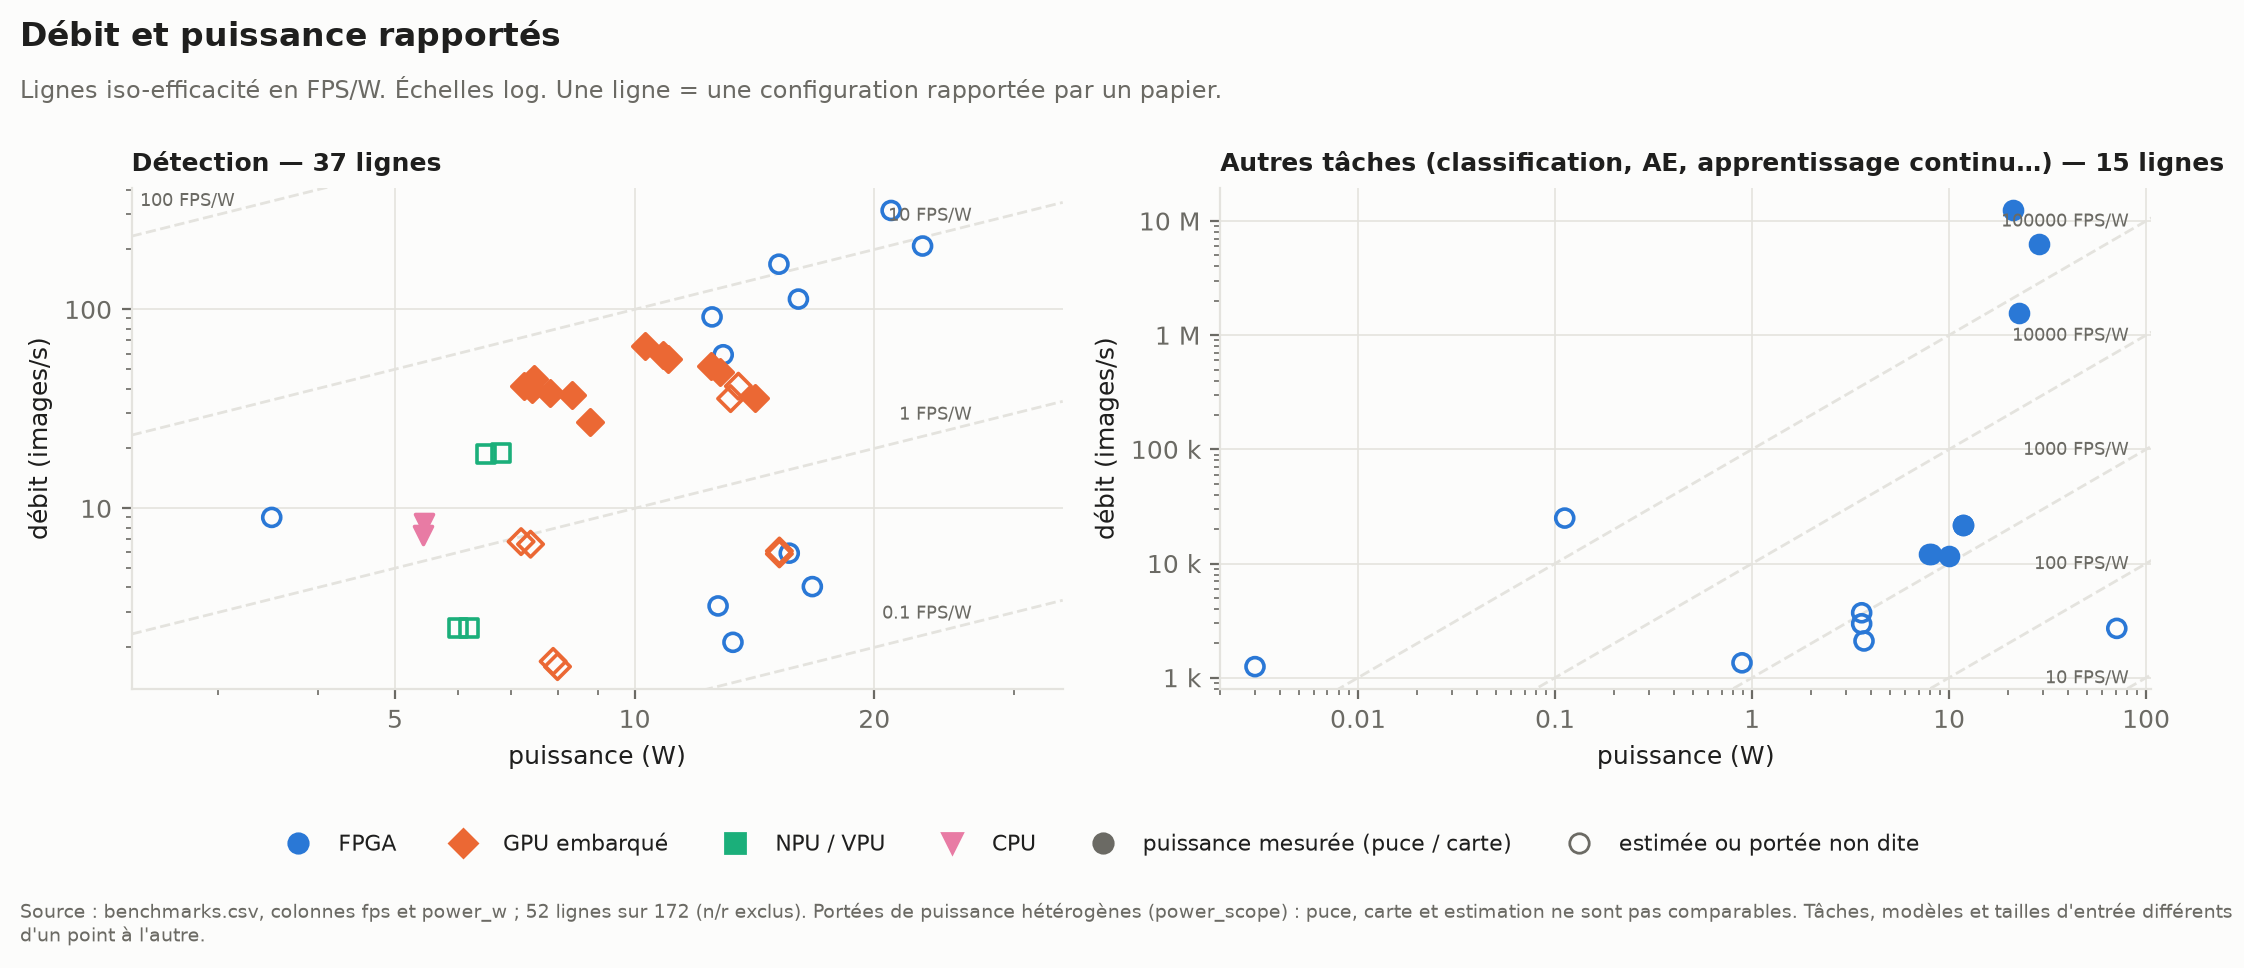
\includegraphics[width=\linewidth]{bench_fps_power.png}
\caption{Sortie de \cmd{pdb plot bench} sur la base fpga : débit et puissance rapportés, une
configuration par point (82 lignes de \cmd{benchmarks.csv} sur 299), la détection à gauche,
les autres tâches à droite. Symboles pleins : puissance mesurée ; creux : estimée ou portée
non précisée. Les points ne sont pas comparables entre eux sans lire la portée de la mesure
(section~\ref{sec:data}, \cmd{bench --comparable}).}
\label{fig:fpspower}
\end{figure}

\paragraph{Déléguer à des sous-agents.}
\label{sec:delegation}
L'agent principal peut confier une tâche à un \gl{sousagent}{sous-agent} qui démarre sans son contexte :
une fiche par agent, un article à extraire, une recherche de \gl{DOI}{DOI}. Les règles du dépôt fixent le
modèle selon la tâche : le plus léger pour la mécanique (ajout, réindexation, contrôle des
métadonnées), un modèle intermédiaire pour la lecture et l'extraction, le plus capable pour
la synthèse et le jugement. Deux agents n'écrivent jamais le même fichier, et
\cmd{benchmarks.csv}, \cmd{INDEX.md} et la réindexation restent à l'agent principal, qui
vérifie ce qu'on lui rapporte. Pour savoir si cela paie, un \gl{hook}{hook} \cmd{SubagentStop} de Claude
Code journalise chaque sous-agent (tokens, coût, durée, outils) dans \cmd{.cache/agents.jsonl},
et \cmd{pdb agents --report} en fait le bilan. Le coût tiré des transcriptions sous-estimait
les tokens de sortie ; il est calé sur le coût que Claude Code compte pour la session. Sur
72 sous-agents journalisés (126~M tokens, 81~\$), la délégation aurait fait économiser
environ 59~\% du coût d'un travail fait en direct. Ce chiffre est une \emph{estimation} :
mêmes tours au tarif de l'agent principal, plus la relecture du travail à chaque tour
suivant.

Pour la caler, une même tâche (trois fiches de lecture de détecteurs YOLO de la base drone)
a été faite deux fois dans des sessions neuves, en direct puis déléguée à trois sous-agents
en parallèle (tableau~\ref{tab:delegation}). Le modèle prédit 2,21~\$ pour la session
directe, qui a coûté 2,30~\$ (écart de 4~\%). La délégation a coûté 41~\% de moins et pris
59~\% de temps en moins. L'essai est unique, et les deux sessions n'ont pas produit le même
travail : en direct, les fiches sont plus longues et comptent 9 lignes de benchmark de plus.
Une part de l'écart vient donc du travail, pas seulement du tarif, et la qualité n'a pas été
notée. L'expérience a aussi fait apparaître un défaut du journal : le hook passait avant
l'écriture du dernier tour du sous-agent, qui manquait au décompte ; il relit désormais la
transcription jusqu'à ce qu'elle soit complète.

\begin{table}[ht]
\centering
\caption{Expérience appariée : trois fiches de lecture, en direct et déléguées (03/10/2026,
un seul essai).}
\label{tab:delegation}
\small
\begin{tabular}{@{}lrr@{}}
\toprule
 & Direct & Délégué \\
\midrule
Coût compté par Claude Code & 2,30~\$ & 1,35~\$ (0,46 + 0,89 pour les sous-agents) \\
Durée & 324\,s & 133\,s \\
Tours de l'agent principal & 29 & 6 (+ 24 pour les 3 sous-agents) \\
Contexte principal en fin de session & 139k tokens & 54k tokens \\
Lignes de \cmd{benchmarks.csv} / taille des fiches & 24 / 23,5k car. & 15 / 17,8k car. \\
\bottomrule
\end{tabular}
\end{table}

\paragraph{État du corpus.} Au 3 octobre 2026, la base fpga compte 101 articles, tous avec
une \gl{fiche}{fiche} terminée, 299 \gl{benchmark}{lignes de benchmark}, 8\,601 passages indexés et 37 lacunes
recensées, dont 29 appuyées par des articles du corpus (sortie de \cmd{pdb status}). Le
corpus a plus que doublé depuis la version précédente de ce texte (45 articles, 3\,479
passages), en grande partie avec des articles sur la sûreté et la certification de l'IA embarquée ;
les fiches et lignes de benchmark des nouveaux articles ont été rédigées par des
sous-agents, puis vérifiées par l'agent principal.

\section{Tests et évaluation}
\label{sec:tests}

\subsection{Tests unitaires}

La suite (\cmd{bin/pdb test}) compte 286 tests répartis en 26 fichiers. Elle s'exécute en
moins de 30 secondes, sans
\gl{GROBID}{GROBID} et sans modèle d'\gl{embedding}{embeddings}, grâce à des substituts déterministes
(tableau~\ref{tab:tests}) :
\begin{itemize}
  \item une vraie sortie \gl{TEI}{TEI} de GROBID (0.8.1), conservée comme fixture, pour le parsing ;
  \item un encodeur et un \gl{crossenc}{cross-encoder} factices, fonctions déterministes du texte, pour
    tester la fusion, le \gl{reranking}{reranking} et l'index incrémental sans sentence-transformers ;
  \item des réponses OpenAlex simulées pour la découverte et l'ajout par \gl{DOI}{DOI} ;
  \item un \gl{PDF}{PDF} synthétique produit par PyMuPDF (une légende suivie d'un tableau à filets)
    pour la reconstruction des tableaux, et des grilles construites à la main pour
    l'appariement des tableaux Docling ;
  \item de petits corpus synthétiques (dont une chaîne de citations datée) pour le graphe et
    la généalogie ;
  \item des bases et un registre temporaires pour la résolution de la base active, la
    création d'une base, le scan et l'import entre bases ;
  \item des transcriptions de sous-agents construites à la main, pour le journal et le calcul
    du coût de la délégation.
\end{itemize}
Les tests de la visualisation et des figures sont ignorés si leurs dépendances optionnelles
ne sont pas installées. Le dernier run (03/10/2026) réussit les 286 tests, y compris celui de
l'acquisition open access, qui échouait au run précédent faute de pouvoir charger le
tokenizer Qwen sans réseau.

\begin{table}[ht]
\centering
\caption{Couverture des tests unitaires (nombre de fonctions de test par fichier).}
\label{tab:tests}
\small
\begin{tabularx}{\linewidth}{@{}lrL@{}}
\toprule
Fichier & Tests & Ce qui est vérifié \\
\midrule
\cmd{test\_plot.py} & 29 & familles de plateformes, classes de précision, exclusion des \nr{}, bloc \cmd{plot} par base, figures périmées, rendu sur la base réelle \\
\cmd{test\_query.py} & 23 & filtres, tri et agrégation de \cmd{bench}, colonnes de source forcées, \cmd{--check}, groupes comparables, identifiants courts, \cmd{paper} \\
\cmd{test\_tables.py} & 19 & reconstruction des tableaux (PDF synthétique), appariement Docling, signaux de qualité, numéros de légende \\
\cmd{test\_schema.py} & 19 & validateurs du modèle de données, colonnes optionnelles, hiérarchie des titres \\
\cmd{test\_rag.py} & 18 & découpage (tableaux par rangées), BM25, fusion, reranking, index incrémental, moteur Qwen simulé, \cmd{verify} et contrôle des nombres \\
\cmd{test\_evaluation.py} & 18 & métriques du banc sur de petits cas construits, notation des réponses finales, emplacements du banc par base \\
\cmd{test\_tei.py} & 12 & parsing d'une sortie GROBID réelle \\
\cmd{test\_openalex.py} & 12 & découverte, ajout par DOI et par liste (réponses simulées) \\
\cmd{test\_base.py} & 12 & base active, \cmd{base.json} minimal, règles invalides, classement, bloc \cmd{plot} \\
\cmd{test\_refs.py} & 11 & rapprochement des références, \cmd{external\_refs.csv}, citations internes \\
\cmd{test\_citation.py} & 11 & exports \cmd{.bib}/\cmd{.ris} : lecture, appariement, priorité \\
\cmd{test\_xbase.py} & 10 & scan entre bases, import (en-tête de la base cible), création d'une base, onglet Bases \\
\cmd{test\_agentlog.py} & 10 & journal des sous-agents : dédoublonnage, réponse incomplète, hook trop précoce relu, issue notée (\cmd{--mark}) \\
\cmd{test\_agentcost.py} & 10 & coût par modèle, calage sur Claude Code, vérification, lectures dupliquées, compaction, économie estimée \\
\cmd{test\_lineage.py} & 9 & généalogie sur une chaîne de citations datée \\
\cmd{test\_graph.py} & 8 & graphe du corpus sur mini-corpus \\
\cmd{test\_bench.py} & 8 & banc synthétique : corpus isolé, localisation des preuves, sortie structurée de \cmd{claude -p}, contrôle du modèle générateur \\
\cmd{test\_ligatures.py} & 7 & réparation des ligatures perdues \\
\cmd{test\_viz.py} & 6 & figures et panneau de détail, sans serveur \\
\cmd{test\_status.py} & 6 & état de la base, tableaux signalés, prochaines actions \\
\cmd{test\_ingest.py} & 6 & conservation des axes, tags et avertissements à la ré-extraction \\
\cmd{test\_claims.py} & 6 & preuves atomiques : schéma, doublons, extrait absent, nombre altéré, mauvais passage \\
\cmd{test\_rag\_qwen.py} & 5 & moteur GPU en mode lexical : sources, conditions numériques, instantané périmé, acquisition isolée \\
\cmd{test\_reindex.py} & 4 & notes sur les benchmarks, mesures propres \\
\cmd{test\_embed.py} & 4 & cache d'embeddings, branchement dans le graphe \\
\cmd{test\_registry.py} & 3 & registre des bases, ordre de résolution de la base active \\
\bottomrule
\end{tabularx}
\end{table}

Deux garde-fous complètent ces tests à l'usage : \cmd{reindex} valide chaque fichier contre
le schéma et s'arrête au premier écart, et une liste de contrôles manuels de la chaîne
d'ingestion (métadonnées, ordre des sections, absence d'en-têtes résiduels, repli sans
GROBID, recoupement des chiffres d'une \gl{fiche}{fiche} avec le PDF) est tenue dans la documentation
technique.

\subsection{Le banc d'évaluation \cmd{pdb eval}}
\label{sec:banc}

Les tests unitaires vérifient que le code fait ce qu'il annonce. Ils ne disent pas si
l'extraction est bonne ni si la recherche trouve les bons \gl{passage}{passages}. \cmd{bin/pdb eval} le
mesure sur le corpus réel, sans \gl{LLM}{LLM} ni réseau, et sans rien écrire dans la base. Il couvre
quatre volets : l'extraction, la recherche, la vérification des citations et les temps ; un
cinquième, les réponses rédigées, est décrit en section~\ref{sec:answers}.
Un run complet prend quelques minutes sur \gl{CPU}{CPU}. \cmd{--save} enregistre le rapport en \gl{JSON}{JSON}
(daté, avec le commit mesuré), et \cmd{--compare} signale les écarts avec le dernier rapport,
avec un code d'erreur si un seuil de \cmd{eval/thresholds.json} n'est plus atteint. La
démarche est la suivante : enregistrer avant un changement (extraction, découpage, modèle,
fusion), le faire, puis comparer. Le banc porte sur la base active : une base peut avoir ses
propres jeux de questions et ses seuils, et ses rapports sont enregistrés dans son dossier
(section~\ref{sec:drone}). Les chiffres ci-dessous portent sur la base fpga et proviennent
d'un run du 03/10/2026 sur 101 articles et 8\,601 passages
(\cmd{bases/fpga/eval/results/2026-10-03T2340-3925690.json}). Ils sont comparés, entre
parenthèses, au run de référence du 28/09 sur 45 articles et 3\,479 passages
(\cmd{2026-09-28T1039-76dc85e}) : les jeux de questions n'ont pas changé, mais le corpus a
plus que doublé et le code a évolué (découpage des tableaux, moteur de recherche
restructuré). Un écart entre les deux runs mêle donc ces deux causes.

\subsection{Qualité de l'extraction}

Le banc calcule d'abord des métriques intrinsèques, qui ne demandent aucune annotation. Il
réutilise ensuite deux vérités terrain déjà présentes dans la base : les métadonnées
vérifiées à la main et les valeurs relevées dans \cmd{benchmarks.csv}
(tableau~\ref{tab:extraction}).

\begin{table}[ht]
\centering
\caption{Qualité de l'extraction (101 articles, tous extraits par GROBID ; entre parenthèses, le run sur 45 articles).}
\label{tab:extraction}
\small
\begin{tabularx}{\linewidth}{@{}Ll@{}}
\toprule
Métrique & Valeur \\
\midrule
Couverture du texte : part des mots du PDF (bibliographie exclue) retrouvés dans \cmd{fulltext.md} & moy. 0,90 ; min. 0,57 (0,91 ; 0,81) \\
Tableaux dont le corps a été extrait (584 tableaux, dont 110 reconstruits par Docling et 11 par PyMuPDF) & 0,78 (0,88) \\
Ligatures restantes, pour 10\,000 mots & 0,00 \\
Articles dont des sections numérotées n'ont pas été détectées & 31 / 101 (13 / 45) \\
En-tête GROBID seul contre \cmd{metadata.json} : titre / année / DOI / arXiv & 0,87 / 0,47 / 0,65 / 0,82 \\
En-tête GROBID seul : F1 sur les noms d'auteurs & 0,84 (0,86) \\
Valeurs de \cmd{benchmarks.csv} retrouvées dans le tableau cité (1\,044 valeurs) & 0,70 (0,65) \\
\quad idem, lignes qui ne citent que des tableaux (682 valeurs) & 0,74 (0,71) \\
Valeurs de \cmd{benchmarks.csv} retrouvées n'importe où dans le texte & 0,79 (0,76) \\
\bottomrule
\end{tabularx}
\end{table}

\begin{itemize}
  \item \emph{La couverture} ne peut pas atteindre 1 : en-têtes, affiliations, texte des
    figures vectorielles et mots coupés par une césure sont exclus volontairement. Elle se
    lit en relatif, d'un run ou d'un article à l'autre. Le minimum (0,57) est une thèse de
    103 pages ; les deux suivants sont des documents réglementaires de l'agence européenne
    de la sécurité aérienne (EASA), entrés avec l'axe sûreté et certification.
  \item \emph{L'année et le DOI} sont bas surtout par construction : le PDF arXiv ne porte
    souvent ni date ni DOI de la version publiée. C'est pour cela que l'ingestion les
    complète depuis arXiv et depuis les exports de citation. Le banc a aussi révélé un vrai
    défaut, encore ouvert : un DOI gabarit d'éditeur (MDPI) n'est pas rejeté.
  \item \emph{Tableaux.} La part des tableaux avec corps baisse (0,88 $\rightarrow$ 0,78), et
    la baisse vient entièrement des 56 nouveaux articles : les 45 anciens gardent 25 tableaux
    sans corps sur 233, les nouveaux en ont 103 sur 351, dont 29 dans les deux documents de
    l'EASA. Docling avait
    fait passer cette part de 0,66 à 0,90 sur 28 articles, avec \gl{OCR}{OCR} pour les tableaux publiés
    en image ; mais la qualité des tableaux passés par l'OCR est inégale (un contrôle à l'œil
    de trois tableaux en trouve un propre, un incomplet et un en partie illisible), d'où la
    mention «~à vérifier~». Les signaux de qualité (section~\ref{sec:archi}) signalent 255
    tableaux sur 584 : 163 au nombre de cellules irrégulier, 107 aux nombres collés, 82 aux
    cellules vides, 14 aux caractères d'OCR douteux. Les échantillons relus de ces deux
    dernières catégories sont de vrais défauts (trois valeurs dans une cellule, premières
    lettres perdues). Le taux «~avec corps~» mesure la présence d'un corps, pas l'exactitude
    des cellules : une vérité terrain par tableau reste à construire.
  \item \emph{Les valeurs retrouvées remontent} (0,65 $\rightarrow$ 0,70 dans le tableau cité)
    après une baisse au passage de 28 à 45 articles. Les lignes de benchmark des nouveaux
    articles sont donc, en moyenne, mieux ancrées dans leur tableau. Le banc ne dit pas si
    une valeur manquante vient de l'extraction ou de la transcription faite par l'\gl{agent}{agent} ;
    c'est ce que \cmd{bench --check} contrôlera ligne par ligne, quand les lignes porteront
    leur passage (\cmd{chunk\_id}) : aucune ne le fait encore.
\end{itemize}

\subsection{Recherche de passages}
\label{sec:eval}

\paragraph{Jeux de questions.} Chaque question est associée aux sections pertinentes du
corpus (identifiées par \cmd{article\#ordre}, indépendamment du découpage en fenêtres).
Ces sections sont choisies par motif textuel dans les articles cibles (par exemple
\emph{reuse factor} dans les deux articles hls4ml). Les questions reformulent le sujet sans
reprendre le motif quand c'est possible : «~removes duplicate bounding boxes~» pour la
non-maximum suppression. Il y a trois jeux :
\begin{itemize}
  \item \emph{dev} : 20 questions en anglais, qui ont servi aux choix de conception (modèle,
    fusion, reranking) ;
  \item \emph{\gl{holdout}{holdout}} : 25 questions en anglais, écrites ensuite et jamais utilisées pour
    régler quoi que ce soit. Elles couvraient les 12 articles absents du jeu dev et
    comprennent 2 questions sur des tableaux et 3 questions qui portent sur plusieurs
    articles. Trois attentes ont été élargies après lecture des passages renvoyés, parce que
    ces passages répondaient bien à la question (avant cela : \gl{recall}{recall@5} de 0,68 avec
    reranking) ;
  \item \emph{FR} : 8 questions du jeu dev traduites à la main en français.
\end{itemize}
Ces jeux ont été écrits pour un corpus de 28 à 45 articles. Sur les 101 actuels, environ
60~\% des articles ne sont visés par aucune question.

\paragraph{Métriques.} recall@5 et recall@10 (au moins une section attendue parmi les 5 ou
10 premiers passages), \gl{MRR}{MRR} (inverse du rang de la première bonne section), \gl{nDCG}{nDCG}@10 à gain
binaire \citep{jarvelin2002ndcg}, qui récompense le fait de trouver \emph{plusieurs}
sections pertinentes, et \gl{paperk}{paper@5} (au moins un passage d'un article cible parmi les 5
premiers).

\begin{table}[ht]
\centering
\caption{Recherche de passages sur 8\,601 passages (101 articles, modèle bge-small-en-v1.5),
le 03/10/2026 ; entre parenthèses, le recall@5 du run sur 45 articles. En gras : meilleure
valeur par jeu.}
\label{tab:eval}
\small
\begin{tabular}{@{}llccccc@{}}
\toprule
Jeu & Mode & recall@5 & recall@10 & MRR & nDCG@10 & paper@5 \\
\midrule
dev (20)     & lexical (BM25)      & 0,85 (0,95) & 0,90 & 0,66 & 0,32 & 0,90 \\
             & dense               & \textbf{0,90} (0,90) & 0,90 & 0,69 & 0,34 & 0,90 \\
             & hybride (défaut)    & 0,80 (0,90) & 0,90 & 0,67 & 0,34 & 0,90 \\
             & hybride + reranking & \textbf{0,90} (1,00) & \textbf{0,95} & \textbf{0,76} & \textbf{0,38} & \textbf{0,95} \\
\midrule
holdout (25) & lexical (BM25)      & 0,56 (0,60) & 0,64 & 0,50 & 0,23 & 0,60 \\
             & dense               & 0,64 (0,64) & 0,64 & 0,49 & 0,29 & 0,76 \\
             & hybride (défaut)    & 0,68 (0,72) & 0,68 & 0,56 & 0,26 & 0,72 \\
             & hybride + reranking & \textbf{0,72} (0,80) & \textbf{0,72} & \textbf{0,62} & \textbf{0,31} & \textbf{0,80} \\
\midrule
FR (8)       & lexical (BM25)      & 0,00 (0,12) & 0,38 & 0,05 & 0,03 & 0,25 \\
             & dense               & \textbf{0,50} (0,62) & 0,50 & 0,26 & 0,12 & \textbf{0,62} \\
             & hybride (défaut)    & \textbf{0,50} (0,50) & \textbf{0,62} & \textbf{0,29} & \textbf{0,13} & \textbf{0,62} \\
             & hybride + reranking & 0,38 (0,50) & 0,50 & \textbf{0,29} & 0,10 & \textbf{0,62} \\
\bottomrule
\end{tabular}
\end{table}

\begin{figure}[ht]
\centering
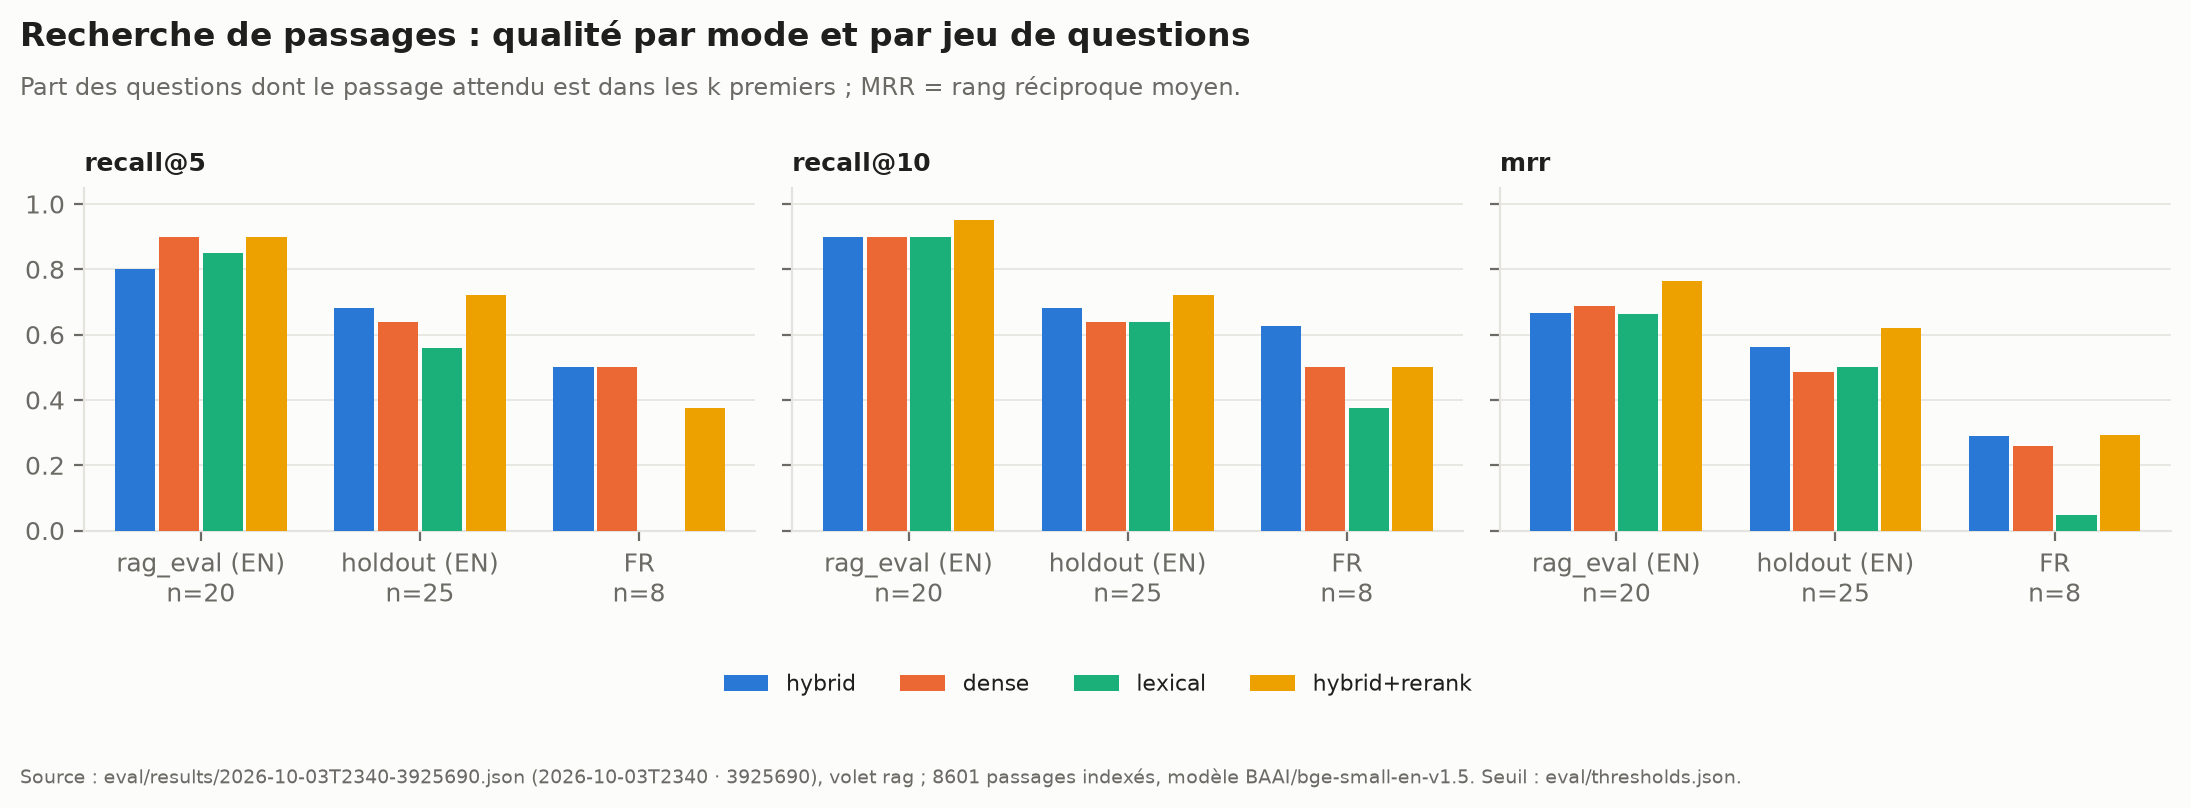
\includegraphics[width=\linewidth]{eval_retrieval.png}
\caption{Les chiffres du tableau~\ref{tab:eval}, tracés par \cmd{pdb plot eval} à partir du
rapport JSON du banc. La ligne pointillée est le seuil d'acceptation (recall@5 $\geq$ 0,8).}
\label{fig:evalretrieval}
\end{figure}

\paragraph{Lecture des résultats.}
\begin{itemize}
  \item \emph{Le holdout passe sous le seuil.} Avec 101 articles, plus aucun mode n'atteint
    un recall@5 de 0,8 sur le holdout : le meilleur, l'hybride avec reranking, tombe de 0,80
    à 0,72, soit deux questions de moins. Le jeu dev perd aussi (1,00 $\rightarrow$ 0,90),
    comme le français (0,50 $\rightarrow$ 0,38). C'est le résultat le plus important de ce
    run, et sa cause n'est pas établie : le corpus a plus que doublé, ce qui ajoute des
    passages voisins des passages attendus ; les tableaux sont désormais indexés par
    rangées ; et le code de recherche a été restructuré. Le seul changement mesuré isolément,
    le découpage des tableaux, ne modifie ni le dev ni le holdout. Le diagnostic prévu rejoue
    les jeux sur l'index restreint aux 45 articles du run de référence, puis l'ancien code sur
    le corpus actuel, pour séparer l'effet du corpus de celui du code. Le seuil n'est pas
    abaissé, et rien n'est réglé sur le holdout.
  \item \emph{Le jeu dev était optimiste.} Sur le holdout, le recall@5 perd 12 à 29 points
    selon le mode, et le lexical est le plus faible. Cela confirme le biais attendu : sur le jeu dev, les sections attendues
    avaient été choisies par mots-clés, ce qui avantageait \gl{BM25}{BM25}.
  \item \emph{Le reranking reste le meilleur mode en anglais}, sur les deux jeux. Il ne
    compense plus, à lui seul, la concurrence des nouveaux articles.
  \item \emph{Échecs réels du holdout} (avec reranking) : la tolérance aux radiations (deux
    questions), l'entraînement quantifié, la mémoire
    d'exemples passés, la distillation de jeu de données, et les deux questions sur des
    tableaux (ressources des autoencodeurs d'un article hls4ml, prototypes de FINN). Pour ces
    deux dernières, le constat initial («~le texte d'un tableau se réduit à sa légende~») ne
    tient plus : depuis Docling, ces tableaux ont un corps et sont assez courts pour ne pas
    être découpés. L'échec vient du vocabulaire : la question dit «~resource utilization~»,
    «~throughput~», «~autoencoder~» ; le tableau dit «~LUT~», «~Thr.put~», «~AE~». Préfixer
    les passages de tableau du titre de l'article a été essayé, et n'aide pas.
  \item \emph{En français, le lexical s'effondre} (recall@5 de 0,00), et l'\gl{index}{index dense}
    résiste mieux, alors que le modèle n'est pas conçu comme multilingue. Le
    reranking, entraîné sur \gl{MSMARCO}{MS MARCO} en anglais, dégrade le classement. Le moteur \gl{GPU}{GPU}
    (section~\ref{sec:qwen}) faisait nettement mieux sur ce jeu.
  \item \emph{Décisions.} L'hybride reste le mode par défaut de \cmd{pdb search}, parce que le
    reranking dégrade le français, selon une règle fixée avant la mesure. \cmd{/paper-ask}
    l'active, parce qu'il formule toujours ses requêtes en anglais et que le rang de la
    première bonne réponse compte quand on n'ouvre que 2 ou 3 passages.
\end{itemize}

Lors d'une mesure antérieure (25/09/2026, jeu dev), le modèle \cmd{all-MiniLM-L6-v2}
obtenait un recall@5 de 0,75 en mode dense contre 0,90 pour bge-small, ce qui a motivé le
choix de ce dernier. Le seuil d'acceptation retenu est un recall@5 d'au moins 0,8 en
anglais.

\subsection{Détecter qu'une question sort du corpus}
\label{sec:horscorpus}

Peut-on dire, sans LLM, que la base ne traite pas une question ? Deux jeux de 10 questions
hors corpus (repliement des protéines, blockchain, etc.) ont été écrits : l'un sert à la
calibration, l'autre à la validation. Le second a été écrit avant toute mesure du
cross-encoder. Deux signaux sont mesurés : le meilleur cosinus de la recherche dense, et le
meilleur score du cross-encoder sur les 3 premiers passages. Pour chacun, le seuil est
choisi sur la calibration (jeu dev et premier jeu hors corpus, dont une question à moitié
couverte par le corpus a été écartée), en maximisant l'exactitude
équilibrée, puis appliqué tel quel à la validation (holdout et second jeu hors corpus). La
règle d'adoption a été fixée avant la mesure : en validation, au moins 80~\% des questions
hors corpus signalées, et au plus 5~\% des questions du corpus.

\begin{table}[ht]
\centering
\caption{Signal «~hors corpus~» : part des questions signalées sur la validation (10
questions hors corpus, 25 questions du holdout), base fpga, 101 articles.}
\label{tab:horscorpus}
\small
\begin{tabular}{@{}lcccc@{}}
\toprule
Signal & Seuil & Hors corpus signalées & Corpus signalées à tort & Adopté \\
\midrule
cosinus, seuil initial fixé à la main & 0,60 & 0,00 & 0,00 & -- \\
cosinus, seuil calibré & 0,78 & 0,80 & 0,20 & non \\
cross-encoder, seuil calibré & 2,12 & 0,90 & 0,32 & non \\
\midrule
Qwen3-Reranker-4B, 28 articles (section~\ref{sec:qwen}) & 0,96 & 1,00 & 0,16 & non \\
\bottomrule
\end{tabular}
\end{table}

Aucun signal ne remplit la règle. Avec bge-small, une question hors sujet obtient un
cosinus aussi élevé qu'une question pertinente : le calibrage initial, fait sur quelques
requêtes, ne tenait pas, et l'alerte ne se déclenchait jamais. Le cross-encoder sépare mieux
les médianes, mais certaines questions du corpus tombent très bas, souvent celles où la
recherche échoue déjà. L'alerte a donc été retirée de \cmd{pdb search}. Le reranker du
moteur GPU est le signal le plus proche de la règle : il signale les 10 questions hors
corpus, mais aussi 4 des 25 questions du holdout (16~\%, pour 5~\% tolérés). Il n'est pas
adopté non plus. La réponse est venue d'ailleurs : quand c'est l'agent qui juge, sur le
contenu des passages lus, il reconnaît les questions hors corpus
(section~\ref{sec:answers}).

\subsection{Vérification des citations}
\label{sec:evalverify}

Le banc tire 40 passages au hasard (graine fixe) et fabrique quatre sortes de citations :
une phrase exacte, qui doit être acceptée ; la même phrase avec un mot remplacé, puis avec
un chiffre modifié, et une phrase d'un autre article, qui doivent être refusées.
«~Acceptée~» signifie un code de sortie nul (\cmd{OK} ou \cmd{APPROX} dans le passage
indiqué).

\begin{table}[ht]
\centering
\caption{Taux d'acceptation de \cmd{pdb verify}, avant et après le contrôle des nombres. «~Avant~» :
run sur 28 articles ; «~Après~» : run du 03/10 sur 101 articles, dont le tirage aléatoire
diffère (33 phrases à chiffre modifiable au lieu de 38).}
\label{tab:verify}
\small
\begin{tabular}{@{}lccl@{}}
\toprule
Citation & Avant & Après & Statuts après \\
\midrule
exacte (40)            & 1,00 & 1,00 & 40 \cmd{OK} \\
chiffre modifié (33)   & \textbf{1,00} & \textbf{0,00} & 33 \cmd{NOMBRES} \\
mot remplacé (40)      & 0,97 & 0,97 & 39 \cmd{APPROX}, 1 \cmd{NOMBRES} \\
d'un autre article (40) & 0,00 & 0,00 & 40 \cmd{ABSENT} \\
\bottomrule
\end{tabular}
\end{table}

Avant le contrôle, \cmd{verify} acceptait toutes les citations dont un chiffre avait été
modifié, alors que les règles de travail de l'agent comptent sur lui pour garantir les
nombres cités. Une première version du contrôle en laissait encore passer 6 (un «~4~»
reconnu dans «~6.4~», un «~2~» trouvé ailleurs dans le passage). L'exigence des mots
voisins règle ces deux cas, mais pas tous. Sur la base drone (section~\ref{sec:drone}), le
run du 03/10 accepte, pour la première fois, une citation au chiffre modifié : «~before
step~2~» au lieu de «~before step~4~», dans un passage qui contient ailleurs «~in step~2
and~3~». Le nombre modifié et son mot voisin existent bien dans le passage, mais pas à cet
endroit. Ce cas n'est pas corrigé ; il montre que le contrôle garantit la présence de chaque
nombre avec son contexte immédiat, pas sa position dans la phrase. Reste aussi non traité :
un \emph{mot} remplacé loin de tout nombre donne toujours \cmd{APPROX}. C'est pourquoi
\cmd{/paper-ask} ne garde une citation \cmd{APPROX} que présentée comme une paraphrase.

\subsection{Temps d'exécution}

\begin{table}[ht]
\centering
\caption{Temps mesurés sur la base fpga (8\,601 passages ; médianes de 3 répétitions, CPU sans GPU).}
\label{tab:temps}
\small
\begin{tabularx}{\linewidth}{@{}Ll@{}}
\toprule
Mesure & Valeur \\
\midrule
Extraction hors GROBID, par article (TEI $\rightarrow$ texte, ligatures, tableaux) & 0,01 à 0,13\,s \\
Chargement de l'index (8\,601 passages, 17\,Mo) & 0,52\,s \\
Encodage bge-small & 18 passages/s ; index complet $\approx$ 491\,s \\
\cmd{search} à chaud, p50 / p95 : lexical & 25 / 31\,ms \\
\quad dense & 117 / 146\,ms \\
\quad hybride & 115 / 168\,ms \\
\quad hybride + reranking & 1\,430 / 1\,782\,ms \\
\cmd{verify} à chaud & 2\,ms \\
Commandes à froid, démarrage de Python compris : \cmd{status} & 0,61\,s \\
\quad \cmd{bench}, \cmd{paper} & 0,09 et 0,08\,s \\
\quad \cmd{show} & 0,75\,s \\
\quad \cmd{search} & 6,6\,s \\
\bottomrule
\end{tabularx}
\end{table}

Le coût d'une recherche vient presque entièrement du démarrage (import de PyTorch,
chargement du modèle) : 6,6\,s à froid contre 0,1\,s à chaud. C'est le coût réel d'un appel
par l'agent, qui lance une commande à chaque fois. Avec 2,5 fois plus de passages qu'au
run du 28/09, les temps de recherche à chaud n'ont presque pas bougé, et le chargement de
l'index passe de 0,29 à 0,52\,s. Le temps de \cmd{verify}, qui était passé de 4 à 246\,ms
sans explication, est revenu à 2\,ms.

\subsection{Essai réel de bout en bout}

Question posée à \cmd{/paper-ask}, sur le corpus de 28 articles : «~comment les papiers
mesurent-ils la puissance, et est-ce comparable ?~». L'agent a enchaîné une requête
\cmd{bench} (57 lignes, 8 articles), une recherche de 10 passages, la lecture de 3 d'entre
eux, 7 vérifications de citations et 8 requêtes d'identité. L'ensemble représente environ
9\,Ko lus, soit environ 2\,500 tokens, sans ouvrir de texte intégral. Les 7 citations
textuelles sont revenues \cmd{OK} au premier essai. La recherche a retrouvé en une requête
les quatre protocoles de mesure du corpus (PMBus et prise murale, multimètre à l'entrée de la
carte, \cmd{tegrastats}, puissance au repos mesurée avant les tests). La structure Lu /
Déduit / Non trouvé a fait ressortir deux points à vérifier dans la base elle-même, dont un
article qui décrit une mesure soignée sans qu'aucune ligne de puissance n'ait été saisie.
L'essai a aussi révélé deux défauts, corrigés depuis et couverts par un test chacun : un
identifiant court tronqué pour un nom d'auteur composé, et une agrégation qui demandait un
script externe (d'où \cmd{bench --count}). Cet essai était unique et jugé par l'agent qui
l'avait exécuté ; la section suivante le remplace par une évaluation répétable.

\subsection{Évaluer la réponse rédigée}
\label{sec:answers}

Les volets précédents mesurent le classement des passages. Ils ne disent pas si la réponse
finale reconnaît une question hors corpus, si ses citations tiennent, ni si elle retrouve
les sources et les valeurs attendues. \cmd{pdb eval --answers} le mesure, toujours sans LLM :
les réponses sont produites à part, puis notées.

\paragraph{Protocole.} Chaque question d'un jeu de réponses porte une catégorie, les
\gl{exigence}{exigences} d'une réponse complète, les sources attendues (sections ou articles), les
valeurs attendues avec leur unité, et le verdict attendu. Il y a quatre catégories : un fait
sourcé dans un article (\emph{simple}), des valeurs avec leurs conditions
(\emph{numérique}), une synthèse sur plusieurs articles (\emph{synthèse}), et une question
proche du thème mais que le corpus ne couvre pas (\emph{absent} : polypes en endoscopie,
langue des signes, sonar, EEG\ldots, vérifiés absents par recherche plein texte). La skill
\cmd{/eval-answers} confie chaque question à un sous-agent qui ne reçoit que son texte, ni
catégorie, ni sources, ni verdict attendu, et qui répond par \cmd{/paper-ask --record}. La
réponse enregistrée est une liste d'affirmations marquées lues ou déduites, chacune avec ses
citations et leurs extraits. Le banc calcule l'exactitude du verdict, la part des citations
acceptées (\cmd{verify} renvoie \cmd{OK} ou \cmd{APPROX} dans le passage indiqué, ou la
section citée figure parmi les sources des lignes de \cmd{bench} de l'article), la part des
affirmations «~lues~» sans aucune citation acceptée, et le rappel des sources et des valeurs
attendues. Une grille de notes humaines (exigences, soutien, conditions, limites, de 0 à 2)
est prévue : les contrôles automatiques vérifient que les extraits existent, pas qu'ils
soutiennent la phrase.

\paragraph{Premiers runs.} Les jeux de départ de la base fpga comptent 12 questions de
développement et 12 réservées, 3 par catégorie, écrites par l'auteur du code. Deux runs ont
été faits le 02/10/2026, une réponse par question, par des sous-agents Sonnet ; le second
avec la version de \cmd{/paper-ask} qui pose les exigences et le verdict de suffisance
(section~\ref{sec:paperask}). Les deux runs ont été faits dans une configuration dégradée :
les modèles de la recherche dense et du reranking n'étaient pas téléchargeables depuis le
conteneur, et la recherche était donc lexicale seule (tableau~\ref{tab:answers}).

\begin{table}[ht]
\centering
\caption{Réponses rédigées, base fpga (12 + 12 questions, recherche lexicale seule). Entre
parenthèses : premier run, avant le verdict de suffisance.}
\label{tab:answers}
\small
\begin{tabularx}{\linewidth}{@{}l*{5}{>{\centering\arraybackslash}X}@{}}
\toprule
Jeu & Verdict juste & Citations acceptées & Affirmations non soutenues & Sources attendues & Valeurs attendues \\
\midrule
dev (12)     & 0,75 (0,83) & 1,00 (0,96) & 0,00 (0,02) & 0,87 (0,91) & 1,00 (1,00) \\
holdout (12) & 0,83 (0,92) & 1,00 (1,00) & 0,00 (0,00) & 0,50 (0,67) & 1,00 (1,00) \\
\bottomrule
\end{tabularx}
\end{table}

\begin{itemize}
  \item \emph{Hors corpus.} Aux deux runs, les 6 questions \emph{absent} sont reconnues comme
    telles, et aucune question du corpus n'est déclarée absente à tort. Les réponses disent
    que la base ne traite pas le sujet, sans le combler par des connaissances générales.
    C'est ce qu'aucun score de recherche ne permettait d'obtenir
    (section~\ref{sec:horscorpus}). Avec 6 questions, c'est un signal, pas une mesure.
  \item \emph{Citations.} Au second run, toutes les citations sont acceptées et toute
    affirmation «~lue~» en porte au moins une.
  \item \emph{Synthèse.} C'est la catégorie faible : 3 verdicts justes sur 6 au premier run,
    2 au second. L'agent répond \cmd{partiel} là où le jeu attend \cmd{suffisant}, parce
    qu'une exigence de la question (budget mémoire de chaque méthode, comparabilité des
    mesures) n'est couverte qu'en partie par le corpus. Ces réponses sont défendables ; la
    frontière entre suffisant et partiel est à préciser dans le jeu plutôt que dans la skill.
    La baisse du verdict juste au second run vient de là, et d'une réponse où la règle
    nouvelle (un verdict \cmd{suffisant} exige que toutes les exigences soient couvertes)
    corrige une incohérence du premier run.
  \item \emph{Variance.} 22 verdicts sur 24 sont identiques d'un run à l'autre : le banc
    est assez stable pour comparer des versions de la skill sur les verdicts. Il ne l'est
    pas encore sur le rappel des sources (0,67 $\rightarrow$ 0,50 sur le holdout sans
    changement de la recherche). Ce rappel sous-estime d'ailleurs les réponses : la plupart
    des écarts viennent d'une source équivalente (la ligne de \cmd{bench} ou le passage du
    tableau plutôt que la section de texte attendue).
\end{itemize}
Aucun seuil n'est encore fixé : il manque un run en recherche hybride avec reranking, des
jeux plus grands (40 questions de développement et 60 réservées par base, écrites ou relues
par un tiers) et les notes humaines.

\subsection{Un second corpus : la base drone}
\label{sec:drone}

La base drone (section~\ref{sec:bases}) a ses propres jeux de questions, écrits selon le même
protocole sur ses 73 premiers articles : 20 questions de développement, 20 réservées, 8 en
français et deux jeux de 10 questions hors corpus. Les seuils sont ceux de la base fpga,
fixés avant le premier run. Le tableau~\ref{tab:drone} compare les deux bases (runs du
03/10/2026 au commit 3925690).

\begin{table}[ht]
\centering
\caption{Banc d'évaluation sur les deux bases qui ont des jeux de questions, le 03/10/2026
(recall@5 sauf mention).}
\label{tab:drone}
\small
\begin{tabularx}{\linewidth}{@{}Lll@{}}
\toprule
Mesure & fpga (101 articles) & drone (87 articles) \\
\midrule
Passages & 8\,601 & 5\,361 \\
Couverture du texte : moyenne / minimum & 0,90 / 0,57 & 0,91 / 0,77 \\
Tableaux avec corps & 0,78 & 0,79 (0,90 sur les 73 articles GROBID) \\
En-tête : titre / année / DOI & 0,87 / 0,47 / 0,65 & 0,92 / 0,64 / 0,70 \\
Valeurs de \cmd{benchmarks.csv} retrouvées dans le tableau cité & 0,70 (1\,044) & 0,62 (739) \\
Dev, hybride / hybride + reranking & 0,80 / 0,90 & 0,90 / 1,00 \\
Réservé, hybride / hybride + reranking & 0,68 / 0,72 (25 q.) & 0,90 / 0,95 (20 q.) \\
Réservé, MRR hybride + reranking & 0,62 & 0,89 \\
Français, hybride + reranking & 0,38 & 0,50 \\
Pertinence faible (\cmd{cos}) : hors corpus / corpus signalés & 0,80 / 0,20 & 1,00 / 0,10 \\
\cmd{verify} : exacte / mot remplacé / chiffre modifié / autre article & 1,00 / 0,97 / 0,00 / 0,00 & 1,00 / 0,82 / 0,03 / 0,00 \\
\bottomrule
\end{tabularx}
\end{table}

La lecture demande de la prudence :
\begin{itemize}
  \item \textbf{Le jeu réservé drone tient son seuil}, mais l'on ne peut pas en conclure que
    la recherche y marche mieux. Le corpus drone est plus hétérogène (détection, suivi,
    neuromorphique, course de drones) : un fait distinctif y a moins de voisins proches que
    dans un corpus centré sur les accélérateurs. Deux attentes ont en outre été élargies
    après lecture des passages renvoyés. Sur 20 questions, 0,05 correspond à une question.
    Entre le 28/09 et le 03/10, avec 14 articles et 836 passages de plus, l'hybride perd une
    question sur chaque jeu anglais, et le reranking n'en perd aucune.
  \item \textbf{Les échecs sont de même nature} que sur la base fpga : un tableau (puissance
    au repos de plusieurs cartes) manqué par tous les modes, et la moitié des questions
    françaises.
  \item \textbf{La pertinence faible reste inutilisable} : le cosinus signale toutes les
    questions hors corpus de validation, mais aussi 2 des 20 questions réservées, au-delà des
    5~\% de fausses alertes tolérés.
  \item \textbf{Les tableaux.} Le passage de Docling sur cette base (29/09) a fait monter la
    part des tableaux avec corps de 0,71 à 0,90 et les valeurs retrouvées dans leur tableau
    de 3 points, à corpus constant : c'est le premier gain de Docling mesuré sur ces valeurs.
    La part retombe à 0,79 sur 87 articles parce que les 14 articles ajoutés depuis l'ont été
    sans leur PDF : extraits par PyMuPDF sans GROBID, ils n'ont aucun tableau avec corps
    (0 sur 50) et ne peuvent pas passer par Docling.
  \item \textbf{\cmd{verify}} accepte une citation au chiffre modifié sur 30, et le seuil
    correspondant n'est plus atteint (section~\ref{sec:evalverify}).
\end{itemize}

\paragraph{La base stage.} Elle n'a pas encore de jeux de questions : le banc ne mesure que
son extraction (56 articles, 3\,640 passages, run \cmd{bases/stage/eval/results/2026-10-03T2344-3925690.json}).
La couverture moyenne est de 0,91 (minimum 0,61 pour le reprint numérisé de Mahalanobis,
1936), mais seuls 71~\% des 254 tableaux ont un corps, aucun n'ayant été repris par Docling,
et seules 42~\% des 112 valeurs de \cmd{benchmarks.csv} sont retrouvées dans le tableau cité
(57~\% n'importe où dans le texte) : ces lignes sont les premières à relire. C'est
aussi la seule base où restent des ligatures non réparées (0,37 pour 10\,000 mots).
Sans jeux propres, le banc retombait jusqu'ici en silence sur les questions de la base fpga,
dont le rappel n'a aucun sens ici : ce repli doit devenir un avertissement.

\subsection{Banc synthétique (\cmd{pdb synth})}
\label{sec:synth}

Les jeux précédents sont petits et écrits par l'auteur du système. \cmd{bin/pdb synth}
prépare une évaluation plus large, séparée de la base de travail (\cmd{.cache/bench/}) :
\begin{itemize}
  \item \emph{corpus gelé} de 200 articles, avec des sujets voisins servant de distracteurs ;
    les passages d'ancrage des questions sont filtrés sur le \gl{FPGA}{FPGA}, l'\gl{AI}{IA} embarquée et
    l'accélération matérielle, en excluant introductions et généralités ;
  \item \emph{génération locale} des questions par un modèle ouvert (Qwen3.8-27B quantifié
    en Q6, servi par llama.cpp sur la même RTX 5090), en JSON contraint par un schéma, avec
    graine fixe ; l'identité du modèle servi et chaque citation sont contrôlées ;
  \item \emph{validation sans annotation humaine} : deux sessions indépendantes d'un LLM
    (Codex pour les 200 questions de référence, puis Claude Code en mode non interactif,
    \cmd{claude -p}) contrôlent chaque question ;
  \item \emph{quotas} : 40 questions à un passage, 40 numériques, 50 inter-articles, 30
    intra-article, 20 sur des tableaux et 20 sans réponse dans le corpus ; partage 40~\%
    développement, 60~\% test, sur des ensembles d'articles disjoints, équilibré entre
    anglais et français, et 40 questions déclinées en variantes traduites et abrégées ;
  \item \emph{ablations} : les quatre modes de recherche du moteur GPU et les deux modes
    CPU de \cmd{pdb search} sur les mêmes questions, puis des variantes d'agent exécutées dans
    un bac à sable (bubblewrap, outils de lecture seuls, corpus en lecture seule), notées par
    un juge LLM.
\end{itemize}
Les fiches et transcriptions numériques produites automatiquement forment un corpus
\emph{enrichi} distinct, qui ne sert jamais à écrire les réponses de référence ; une ligne de
benchmark n'y est gardée que si chacun de ses nombres figure dans la section citée. Le
protocole et ses tests sont en place ; ses résultats ne sont pas encore disponibles et ne
sont donc pas rapportés ici.

\subsection{Menaces à la validité}

\begin{itemize}
  \item Les jeux sont petits : sur 25 questions, un écart de 0,04 correspond à une seule
    question, et aucun écart n'est lisible en dessous de deux questions. Le holdout n'a servi
    à régler aucun paramètre, mais il a été écrit, comme le jeu dev, par l'auteur du système.
    Des questions écrites par un tiers sont nécessaires pour confirmer les écarts. Le second
    corpus (section~\ref{sec:drone}) montre que les tendances ne tiennent pas à un seul
    corpus, mais ses questions ont été écrites par le même auteur.
  \item Les jeux n'ont pas suivi la croissance des bases : écrits pour 45 et 73 articles,
    ils interrogent aujourd'hui moins de la moitié du corpus fpga, et la base stage n'en a
    aucun.
  \item Les sections attendues sont choisies par motif textuel. C'est une approximation : une
    bonne réponse formulée autrement, ou trouvée dans un article ajouté après l'écriture du
    jeu, est comptée comme un échec.
  \item La vérité terrain des tableaux ne couvre que les valeurs reprises dans
    \cmd{benchmarks.csv}, et le taux de tableaux «~avec corps~» ne dit rien de l'exactitude
    des cellules.
  \item Les réponses rédigées sont notées automatiquement sur 24 questions, en recherche
    lexicale seule, et les notes humaines n'ont pas encore été attribuées : la validité des
    citations est contrôlée, pas le fait qu'elles soutiennent la phrase.
  \item La comparaison des deux moteurs porte sur le corpus de 28 articles et sur la chaîne
    \cmd{pdb rag} d'origine ; elle n'a pas été refaite avec le moteur intégré à
    \cmd{pdb search}, ni sur le corpus actuel.
  \item L'économie de la délégation repose sur une estimation, calée par un seul essai
    apparié, sur une seule tâche, sans notation de la qualité.
  \item Le banc synthétique aura ses propres biais : questions générées par un LLM, validées
    et notées par d'autres LLM. Il mesurera ce corpus gelé et cette distribution de tâches,
    pas le travail de recherche en général.
\end{itemize}

\section{Limites et perspectives}

\begin{itemize}
  \item \textbf{Passage à l'échelle.} De 45 à 101 articles, le \gl{recall}{recall@5} du \gl{holdout}{holdout} avec
    \gl{reranking}{reranking} passe de 0,80 à 0,72, sous le seuil. Avant tout réglage, il faut séparer
    l'effet du corpus de celui du code, en rejouant les jeux sur le sous-corpus commun et
    l'ancien code sur le corpus actuel. Le plan suivant est spécifié : des jeux propres à
    chaque base, sans repli silencieux ; une taille proportionnelle au corpus (holdout d'au
    moins 40 questions ou la moitié du nombre d'articles) ; des quotas par axe de la base et
    par type de question (tableaux, plusieurs articles) ; des questions proposées par la
    chaîne du banc synthétique et relues par un humain ; un nouveau run de référence à chaque
    croissance de 25~\% du corpus ; et des intervalles de confiance par bootstrap, pour ne
    signaler un écart que s'il en sort.
  \item \textbf{Tableaux.} Ils restent la partie la plus fragile de l'extraction : 22~\% des
    tableaux de la base fpga n'ont pas de corps, environ 40~\% de ceux qui en ont un sont
    signalés par un indicateur de qualité, et les tableaux passés par l'\gl{OCR}{OCR} sont de qualité
    inégale. Les tableaux se retrouvent mal par la recherche, maintenant pour une raison de
    vocabulaire (abréviations des en-têtes) plus que de découpage ; un glossaire
    d'abréviations par base ou des requêtes multiples sont les pistes. Restent à faire : une
    skill de relecture des tableaux signalés, en commençant par ceux que cite
    \cmd{benchmarks.csv}, une vérité terrain d'une vingtaine de tableaux annotés à la main,
    et une OCR ciblée sur la zone du tableau plutôt que sur tout le PDF. Une ré-extraction
    (\cmd{ingest --reparse}) défait aussi certaines réparations de ligatures : à corriger
    avant toute ré-extraction en masse.
  \item \textbf{Comparaisons.} \cmd{bench --comparable} dit quelles lignes se comparent sur un
    axe. Une commande \cmd{pdb compare}, spécifiée, comparera sur deux axes (débit contre
    puissance, à métrique et jeu égaux), donnera un niveau de confiance par groupe et
    expliquera chaque ligne exclue. Les colonnes optionnelles restent à remplir : aucune
    ligne ne porte encore son passage.
  \item \textbf{Preuves atomiques.} Un seul article a ses \cmd{claims.jsonl}. Il reste à les
    produire pour les autres, à les indexer comme renvois vers leur passage, et à les faire
    lire par \cmd{/paper-ask}, qui devrait y gagner sur les questions de synthèse.
  \item \textbf{Réponses.} Il manque un run des réponses en recherche hybride avec reranking,
    des jeux plus grands relus par un tiers, des jeux pour les bases drone et stage, et les
    notes humaines.
  \item \textbf{Questions hors corpus.} Aucun score de recherche ne dit de façon fiable que la
    base ne traite pas le sujet ; le verdict de suffisance de l'agent y parvient sur les 6
    questions testées, ce qui reste à confirmer sur un jeu plus grand.
  \item \textbf{Vérification.} \cmd{verify} refuse les chiffres modifiés quand le nombre et ses
    voisins ne se retrouvent pas ailleurs dans le passage, mais pas dans le cas contraire
    (section~\ref{sec:evalverify}), et un mot remplacé loin de tout nombre passe encore pour
    une paraphrase (\cmd{APPROX}). Le contrôle de \cmd{rag check-answer}, sur la route GPU,
    ne vérifie pas encore les nombres.
  \item \textbf{Métadonnées.} Un \gl{DOI}{DOI} gabarit d'éditeur (MDPI) n'est pas encore rejeté à
    l'extraction ; il est corrigé à la main dans la base, mais un nouvel article du même
    éditeur en hériterait.
  \item \textbf{Langue.} Corpus et modèle par défaut sont en anglais, et la recherche sur
    \gl{CPU}{CPU} perd beaucoup en français (recall@5 de 0,38 avec reranking). Le moteur \gl{GPU}{GPU}
    retrouvait les 8 questions françaises, au prix d'un GPU. Pistes spécifiées : traduire
    systématiquement la requête et fusionner les résultats, évaluer un modèle multilingue à
    côté du modèle actuel, et porter le jeu français à 30 questions par base.
  \item \textbf{Provenance.} Rien ne garde trace de l'état du corpus sur lequel une réponse a
    été rédigée : après une réindexation, on ne peut pas savoir sur quoi elle reposait. Une
    empreinte du corpus et un journal des réponses sont prévus.
  \item \textbf{Latence.} Environ 7\,s par \cmd{search} à froid, contre 0,1\,s à chaud,
    dues pour l'essentiel à l'import de PyTorch et au chargement du modèle ; \cmd{show} et
    \cmd{verify}, qui s'en passent, répondent en moins d'une seconde. Un processus résident, par exemple
    un serveur \gl{MCP}{MCP} exposant les mêmes commandes, ne paierait ce coût qu'une fois, et
    permettrait d'utiliser la base depuis d'autres applications. Le même argument vaut pour
    le moteur GPU, qui recharge ses modèles à chaque requête (3 à 4\,s).
  \item \textbf{Généricité.} Le même code sert trois bases (section~\ref{sec:bases}), dont une
    sans aucune mesure matérielle, et une nouvelle se crée par \cmd{pdb base new}. Les
    colonnes obligatoires de \cmd{benchmarks.csv} (\gl{FPS}{FPS}, \gl{GOPS}{GOPS}, ressources \gl{FPGA}{FPGA}) restent
    marquées par le domaine d'origine : sur 100 lignes, la base stage n'a aucune ressource FPGA et
    deux débits ; elle rapporte ses résultats en précision ou en erreur de prédiction. Les colonnes optionnelles et le bloc
    \cmd{plot} par base ont assoupli le schéma sans le rendre configurable.
\end{itemize}

\section{Conclusion}

PaperDatabase montre qu'un corpus de recherche de taille modeste peut être rendu
exploitable par un \gl{agent}{agent} \gl{LLM}{LLM} sans base de données ni service externe : des fichiers texte
bien structurés, un tableau de chiffres sourcés et une recherche hybride déterministe
suffisent. La génération reste à l'agent, mais tout ce qu'il cite peut être rejoué et
vérifié par une commande. Le coût d'une réponse sourcée baisse d'un ordre de grandeur par
rapport à la lecture des textes intégraux, et déléguer la lecture à des sous-agents moins
coûteux réduit encore la facture, de 41~\% sur le seul essai apparié.

Le banc d'évaluation a montré l'intérêt de mesurer ce que l'on croit acquis : un jeu de
questions optimiste, une alerte qui ne se déclenchait jamais, une vérification qui laissait
passer des chiffres faux, puis, en remesurant, une recherche qui perd du rappel quand le
corpus double. Ce dernier point est le principal problème ouvert. L'évaluation des réponses
rédigées a apporté le résultat inverse : là où aucun score ne savait dire qu'une question
sort du corpus, l'agent le dit quand on l'oblige à confronter chaque exigence de la question
aux passages lus. Le même code sert trois bases isolées, sur lesquelles le banc retrouve les
mêmes forces et les mêmes faiblesses. Les prochaines étapes sont le diagnostic de la baisse
du rappel et des jeux à l'échelle des bases, des questions écrites par un tiers, les notes
humaines des réponses, une meilleure recherche dans les tableaux, la comparaison sur deux
axes et un moteur résident qui évite de recharger les modèles à chaque requête.

\bibliographystyle{plainnat}
\bibliography{refs}

\appendix
\section{Glossaire des acronymes}
\label{sec:acronymes}

\begin{center}
\small
\begin{tabularx}{\linewidth}{@{}lL@{}}
\toprule
Acronyme & Signification \\
\midrule
\hypertarget{gl:API}{API} & \emph{Application Programming Interface}, interface de programmation \\
\hypertarget{gl:BF16}{BF16} & \emph{bfloat16}, format flottant sur 16 bits \\
\hypertarget{gl:BM25}{BM25} & \emph{Best Matching 25}, fonction de score de la recherche lexicale \\
\hypertarget{gl:BRAM}{BRAM} & \emph{Block RAM}, mémoire embarquée d'un FPGA \\
\hypertarget{gl:CPU}{CPU} & \emph{Central Processing Unit}, processeur généraliste \\
\hypertarget{gl:CSV}{CSV / TSV} & \emph{Comma- / Tab-Separated Values}, tableau texte à séparateur virgule / tabulation \\
\hypertarget{gl:DOI}{DOI} & \emph{Digital Object Identifier}, identifiant pérenne d'une publication \\
\hypertarget{gl:DSP}{DSP} & \emph{Digital Signal Processing} : bloc de calcul (multiplieur-accumulateur) d'un FPGA \\
\hypertarget{gl:FPGA}{FPGA} & \emph{Field-Programmable Gate Array}, circuit logique reprogrammable \\
\hypertarget{gl:FPS}{FPS} & \emph{Frames Per Second}, images par seconde \\
\hypertarget{gl:FTS5}{FTS5} & \emph{Full-Text Search} version 5, index plein texte de SQLite \\
\hypertarget{gl:GOPS}{GOPS} & \emph{Giga Operations Per Second}, milliards d'opérations par seconde \\
\hypertarget{gl:GPU}{GPU} & \emph{Graphics Processing Unit}, processeur graphique \\
\hypertarget{gl:GROBID}{GROBID} & \emph{GeneRation Of BIbliographic Data}, extracteur de structure d'articles PDF \\
\hypertarget{gl:AI}{IA} & intelligence artificielle \\
\hypertarget{gl:INT8}{INT8} & entiers sur 8 bits (quantification) \\
\hypertarget{gl:JSON}{JSON} & \emph{JavaScript Object Notation}, format de données texte \\
\hypertarget{gl:LLM}{LLM} & \emph{Large Language Model}, grand modèle de langage \\
\hypertarget{gl:LUT}{LUT} & \emph{Look-Up Table}, cellule logique élémentaire d'un FPGA \\
\hypertarget{gl:MCU}{MCU} & \emph{Microcontroller Unit}, microcontrôleur \\
\hypertarget{gl:MCP}{MCP} & \emph{Model Context Protocol}, protocole d'exposition d'outils à un agent LLM \\
\hypertarget{gl:MRR}{MRR} & \emph{Mean Reciprocal Rank}, moyenne de l'inverse du rang de la première bonne réponse \\
\hypertarget{gl:MSMARCO}{MS MARCO} & \emph{Microsoft MAchine Reading COmprehension}, jeu de données de recherche de passages \\
\hypertarget{gl:nDCG}{nDCG} & \emph{normalized Discounted Cumulative Gain}, qualité d'un classement \\
\hypertarget{gl:NMS}{NMS} & \emph{Non-Maximum Suppression}, suppression des boîtes de détection en double \\
\hypertarget{gl:OCR}{OCR} & \emph{Optical Character Recognition}, reconnaissance optique de caractères \\
\hypertarget{gl:PDF}{PDF} & \emph{Portable Document Format} \\
\hypertarget{gl:RAG}{RAG} & \emph{Retrieval-Augmented Generation}, génération augmentée par recherche \\
\hypertarget{gl:RRF}{RRF} & \emph{Reciprocal Rank Fusion}, fusion de classements par rangs réciproques \\
\hypertarget{gl:SHA}{SHA-1} & \emph{Secure Hash Algorithm 1}, empreinte d'un texte \\
\hypertarget{gl:TEI}{TEI} & \emph{Text Encoding Initiative}, format XML de sortie de GROBID \\
\hypertarget{gl:YOLO}{YOLO} & \emph{You Only Look Once}, famille de détecteurs d'objets \\
\bottomrule
\end{tabularx}
\end{center}

\section{Lexique}
\label{sec:lexique}

\begin{center}
\small
\begin{tabularx}{\linewidth}{@{}lL@{}}
\toprule
Terme & Sens dans ce document \\
\midrule
\hypertarget{gl:agent}{agent} & LLM qui appelle des outils (lecture de fichiers, commandes) pour accomplir une tâche ; ici Claude Code \\
\hypertarget{gl:benchmark}{benchmark (ligne de)} & une configuration rapportée par un article (modèle, plateforme, précision, débit, puissance\ldots), avec sa section source, dans \cmd{benchmarks.csv} \\
\hypertarget{gl:passage}{chunk, passage} & fragment de section indexé pour la recherche, identifié par \cmd{<article>\#<section>.<k>} \\
\hypertarget{gl:crossenc}{cross-encoder} & modèle qui note ensemble une requête et un passage ; sert au reranking \\
\hypertarget{gl:exigence}{exigence} & ce qu'une réponse complète doit établir (valeur, plateforme, condition\ldots) ; statut \cmd{couvert}, \cmd{partiel} ou \cmd{absent} \\
\hypertarget{gl:embedding}{embedding} & vecteur qui représente le sens d'un texte ; deux textes proches ont des vecteurs proches \\
\hypertarget{gl:fiche}{fiche} & lecture critique d'un article (\cmd{fiche.md}) : problème, méthode, résultats, limites, pertinence \\
\hypertarget{gl:hook}{hook} & commande que Claude Code lance d'elle-même à un moment donné (ici, à la fin de chaque sous-agent) \\
\hypertarget{gl:holdout}{holdout} & jeu de questions réservé, qui n'a servi à régler aucun paramètre \\
\hypertarget{gl:index}{index dense / lexical} & index par embeddings (sens) / par mots exacts (BM25, FTS5) \\
\hypertarget{gl:gap}{lacune (gap)} & zone que le corpus ne couvre pas, consignée dans \cmd{gaps.md} \\
\hypertarget{gl:nr}{\texttt{n/r}} & «~non rapporté~» : valeur absente de l'article, jamais estimée \\
\hypertarget{gl:scope}{portée de puissance} & ce que couvre une mesure de puissance (puce, carte, estimation), colonne \cmd{power\_scope} \\
\hypertarget{gl:claim}{preuve atomique (claim)} & une affirmation d'un article, avec son passage source et l'extrait exact qui la porte, dans \cmd{claims.jsonl} \\
\hypertarget{gl:preprint}{preprint} & article diffusé sans relecture par les pairs (arXiv) \\
\hypertarget{gl:recall}{recall@$k$} & part des questions dont une section attendue figure parmi les $k$ premiers passages \\
\hypertarget{gl:paperk}{paper@$k$} & part des questions dont un article attendu figure parmi les $k$ premiers passages \\
\hypertarget{gl:reranking}{reranking} & reclassement des premiers résultats par un modèle plus coûteux \\
\hypertarget{gl:skill}{skill} & procédure écrite que l'agent suit pour une tâche (\cmd{/paper-ask}, \cmd{/paper-fiche}\ldots) \\
\hypertarget{gl:sousagent}{sous-agent} & agent lancé par l'agent principal pour une tâche délimitée, sans son contexte, souvent sur un modèle moins coûteux \\
\hypertarget{gl:toolflow}{toolflow} & chaîne d'outils qui transforme un réseau de neurones en accélérateur matériel (FINN, hls4ml\ldots) \\
\hypertarget{gl:verdict}{verdict de suffisance} & en tête d'une réponse : \cmd{suffisant} (toutes les exigences couvertes), \cmd{partiel} ou \cmd{absent} (aucune) \\
\bottomrule
\end{tabularx}
\end{center}

\section{Commandes}

\begin{center}
\small
\begin{tabularx}{\linewidth}{@{}lL@{}}
\toprule
Commande & Effet \\
\midrule
\cmd{bin/pdb status [--tables]} & état de la base et prochaines actions ; signaux de qualité des tableaux \\
\cmd{bin/pdb add <arxiv | doi | pdf>} & acquisition, ingestion et réindexation \\
\cmd{bin/pdb ingest [--force | --reparse]} & (ré)extraction des PDF de \cmd{inbox/} \\
\cmd{bin/pdb ingest --reparse --tables docling [--ocr]} & tableaux sans corps repris par Docling \\
\cmd{bin/pdb reindex} & \cmd{INDEX.md}, \cmd{external\_refs.csv}, index de passages \\
\cmd{bin/pdb bench [filtres]} & filtre \cmd{benchmarks.csv}, colonnes de source toujours affichées \\
\cmd{bin/pdb bench --check | --comparable | --add-columns} & valeurs retrouvées dans leur passage ; groupes comparables ; colonnes optionnelles \\
\cmd{bin/pdb claims <id> [--check]} & preuves atomiques d'un article et leur contrôle \\
\cmd{bin/pdb paper <id | mot>…} & identité d'un ou plusieurs articles \\
\cmd{bin/pdb search "<q>"} & passages classés (hybride, \cmd{--rerank} en option ; \cmd{--gpu} / \cmd{--cpu}) \\
\cmd{bin/pdb gpu [on | off]} & état du moteur GPU ; activation pour la machine, retour au CPU \\
\cmd{bin/pdb show <chunk\_id>} & texte exact d'un passage \\
\cmd{bin/pdb verify <chunk\_id> "<cit.>"} & contrôle d'une citation \\
\cmd{bin/pdb cites | cited-by <id>} & graphe de citations internes \\
\cmd{bin/pdb discover} & candidats à l'ajout via OpenAlex \\
\cmd{bin/pdb plot [bench | eval | corpus | all]} & figures statiques et \cmd{figures/manifest.json} \\
\cmd{bin/pdb plot --check | --stale} & bloc \cmd{plot} proposé pour la base ; figures périmées seulement \\
\cmd{bin/pdb viz} & visualisation locale du corpus \\
\cmd{bin/pdb rag index | search | evidence | benchmarks} & moteur GPU (Qwen3) : index, recherche, preuves, chiffres \\
\cmd{bin/pdb rag acquire | approve | check-answer} & acquisition open access, import après accord, contrôle d'une réponse \\
\cmd{bin/pdb synth <étape>} & banc synthétique (corpus, génération, validation, ablations, rapport) \\
\cmd{bin/pdb base list | new | register | use} & bases enregistrées, création, enregistrement, base par défaut \\
\cmd{bin/pdb base info | check} & profil et axes d'une base ; effet des règles de \cmd{base.json} \\
\cmd{bin/pdb base scan | import <base>:<id>} & articles utiles d'une autre base ; copie d'un article \\
\cmd{bin/pdb --base <nom> <commande>} & agir sur une autre base que celle du dossier courant \\
\cmd{bin/pdb test} & tests unitaires \\
\cmd{bin/pdb eval [--extract | --rag | --speed]} & banc d'évaluation, par volet ou complet \\
\cmd{bin/pdb eval --save | --compare} & enregistre un rapport ; compare au dernier et aux seuils \\
\cmd{bin/pdb eval --rag --gpu} & recherche évaluée avec le moteur GPU, mêmes clés \\
\cmd{bin/pdb eval --questions | --answers <run>…} & questions seules ; notation des réponses rédigées \\
\cmd{bin/pdb agents [--report | --scan | --mark]} & journal et coût des sous-agents, économie de la délégation \\
\midrule
\cmd{/paper-add}, \cmd{/paper-fiche} & skills de l'agent : ajout ; fiche et lignes de benchmark \\
\cmd{/paper-extract} & preuves atomiques d'un article (\cmd{claims.jsonl}) \\
\cmd{/paper-ask}, \cmd{/paper-gaps}, \cmd{/paper-discover} & réponse sourcée avec verdict de suffisance ; carte des lacunes ; découverte \\
\cmd{/eval-answers} & produit à l'aveugle les réponses d'un jeu, puis les fait noter \\
\cmd{/paper-research} & réponse sourcée avec le moteur GPU et l'acquisition open access \\
\cmd{/base-profile} & proposition d'affinage du profil et des règles de la base \\
\bottomrule
\end{tabularx}
\end{center}

\paragraph{Installation.} Python 3.12 et Docker (pour GROBID) :
\begin{lstlisting}
bash bin/setup.sh                                  # .venv et dépendances
.venv/bin/pip install -r requirements-embed.txt    # optionnel : recherche dense
bin/pdb grobid start                               # GROBID sur localhost:8070
bin/pdb add 2507.18174 && bin/pdb test
\end{lstlisting}

\end{document}
